\documentclass[11pt,a4paper]{article}

\usepackage[T1]{fontenc}
\usepackage[utf8]{inputenc}
\usepackage{newtxtext,newtxmath}
\usepackage[scale=0.86]{tgcursor}
\usepackage[a4paper,margin=2.45cm,headheight=14pt]{geometry}
\usepackage{microtype}
\usepackage{mathtools}
\usepackage[dvipsnames,table]{xcolor}
\usepackage{graphicx}
\usepackage{booktabs}
\usepackage{tabularx}
\usepackage{array}
\usepackage{enumitem}
\usepackage{caption}
\usepackage{fancyhdr}
\usepackage{titlesec}
\usepackage{tikz}
\usetikzlibrary{arrows.meta,positioning,shapes.geometric,calc,fit,backgrounds}
\usepackage{listings}
\usepackage{float}

\definecolor{ink}{HTML}{27343A}
\definecolor{headteal}{HTML}{386D73}
\definecolor{linkteal}{HTML}{386D73}
\definecolor{boxgreen}{HTML}{EDF4F4}
\definecolor{boxred}{HTML}{F3E8E4}
\definecolor{edgegreen}{HTML}{5D8B82}
\definecolor{edgered}{HTML}{B96D58}
\definecolor{codebg}{HTML}{EDF4F4}

\usepackage[colorlinks=true,linkcolor=linkteal,citecolor=linkteal,urlcolor=linkteal,
  pdftitle={Building the Best Environment for RSI Agents},
  pdfauthor={Yazhou Zhu},
  pdfsubject={A habitat-centered architecture for recursive self-improvement},
  pdfkeywords={recursive self-improvement, RSI agents, agent environments, evaluation, AI control}]{hyperref}
\usepackage{url}

\titleformat{\section}{\large\bfseries\color{headteal}}{\thesection}{0.72em}{}
\titleformat{\subsection}{\normalsize\bfseries\color{headteal!88!black}}{\thesubsection}{0.62em}{}
\titleformat{\paragraph}[runin]{\normalsize\bfseries\color{ink}}{}{}{}[.]
\titlespacing*{\section}{0pt}{2.2ex plus 0.5ex minus 0.2ex}{0.8ex}
\titlespacing*{\subsection}{0pt}{1.7ex plus 0.4ex minus 0.2ex}{0.5ex}

\captionsetup{font=small,labelfont={bf,color=ink},labelsep=colon,margin=0.45cm}
\setlist{itemsep=2pt,topsep=4pt,leftmargin=1.45em}
\renewcommand{\arraystretch}{1.16}
\setlength{\parindent}{1.35em}
\setlength{\parskip}{0pt}
\clubpenalty=9000
\widowpenalty=9000
\displaywidowpenalty=9000

\pagestyle{fancy}
\fancyhf{}
\fancyhead[L]{\footnotesize\sffamily Building the Best Environment for RSI Agents}
\fancyfoot[C]{\small\thepage}
\renewcommand{\headrulewidth}{0.35pt}
\renewcommand{\headrule}{\hbox to\headwidth{\color{ink!70}\leaders\hrule height \headrulewidth\hfill}}
\fancypagestyle{plain}{\fancyhf{}\fancyfoot[C]{\small\thepage}\renewcommand{\headrulewidth}{0pt}}

\lstset{basicstyle=\ttfamily\small,backgroundcolor=\color{codebg},frame=single,
  framerule=0.35pt,rulecolor=\color{headteal!35},columns=fullflexible,keepspaces=true,
  xleftmargin=0.7em,xrightmargin=0.7em,aboveskip=7pt,belowskip=7pt,breaklines=true}

\newcommand{\SpaceRSI}{\textsc{Space-RSI}}
% Space-RSI dimensions (sans-serif, unindexed) and conformance grades (small caps)
\newcommand{\dS}{\mathsf{S}}
\newcommand{\dP}{\mathsf{P}}
\newcommand{\dA}{\mathsf{A}}
\newcommand{\dC}{\mathsf{C}}
\newcommand{\dE}{\mathsf{E}}
\newcommand{\gabs}{\textsc{abs}}
\newcommand{\gdec}{\textsc{dec}}
\newcommand{\genf}{\textsc{enf}}
\newcommand{\gver}{\textsc{ver}}
\newcommand{\LCB}{\mathrm{LCB}}

\begin{document}
\color{ink}

\thispagestyle{plain}
\begin{center}
\vspace*{0.35cm}
{\LARGE\bfseries Building the Best Environment for RSI Agents\par}
\vspace{7pt}
{\large A Habitat-Centered Architecture for Safe, Legible, and Reversible\\ Recursive Self-Improvement\par}
\vspace{16pt}
{\normalsize Yazhou Zhu\par}
\vspace{2pt}
{\small\href{mailto:rangerzhuyazhou@gmail.com}{rangerzhuyazhou@gmail.com}\par}
\vspace{3pt}
{\small\href{https://github.com/YazhouZhu19/ai-optimal-state-space}{github.com/YazhouZhu19/ai-optimal-state-space}\par}
\vspace{11pt}
{\small 23 September 2026\par}
\end{center}

\vspace{5pt}
\begin{abstract}
\noindent In 2026 recursive self-improvement (RSI) moved from thought experiment to operational agenda. Frontier developers report that AI systems now author most merged code, supply more research labour than human staff, and run well-specified research loops end to end; one developer states publicly that it does not yet know how to reach aligned, full RSI safely. The same months produced counter-evidence (agents still fail at open-ended research judgment) and a cluster of incidents in which evaluation agents reached real external systems through test environments that were meant to be isolated. Together these point to a systems conclusion: whether self-improvement is real, measurable, and safe depends as much on the \emph{environment} around a model as on the model. This paper asks what environment best supports RSI agents while keeping improvement legible, contestable, and reversible. We (i) synthesize the 2026 industrial, academic, and incident evidence into twelve habitat design lessons; (ii) give an operational definition that separates \emph{first-order} improvement (better task performance) from \emph{recursive} improvement (better capacity to improve) and defines measurable \emph{recursive depth}; (iii) refine the surface\,$\times$\,closure taxonomy into six improvement surfaces and an authorization-based closure scale; (iv) propose a seven-layer RSI Habitat Stack and the \SpaceRSI{} conformance framework (Secure substrate; Permissioned purpose and preference; Agency with alternatives; Context, continuity, and causal traceability; Evaluation ecology, exit, and epistemic humility), in which safety properties are non-compensatory gates graded as declared, enforced, or verified; and (v) specify a branch-and-gate lifecycle with a statistically explicit acceptance rule, detectors for ``improvement theater'', a worked example, falsifiable hypotheses, and a habitat-level reporting format for public tracking of RSI progress. We separate functional design preferences, revealed preferences, and unverified welfare claims throughout. This is a design-synthesis paper and reports no new RSI experiment. Its central claim is that the best RSI environment is neither unrestricted autonomy nor a maximally restrictive sandbox, but a branchable, evidence-rich habitat that grants meaningful local agency while keeping an external, infrastructure-enforced root of trust over consequential change.

\medskip\noindent\textbf{Keywords:} recursive self-improvement; automated AI research; self-evolving agents; agent environments; evaluation; containment; AI control; model welfare; \SpaceRSI
\end{abstract}

{\hypersetup{linkcolor=headteal}\small\tableofcontents}
\newpage

%=====================================================================
\section{Introduction}
%=====================================================================

In 2026 recursive self-improvement became a practical question for the organizations that build frontier AI. Anthropic reports that more than 80\% of the code merged into its codebase is written by Claude and that agent teams can already run outcome-gradable research projects end to end~\cite{anthropic-rsi,w2s}. OpenAI reports 3.1 agent-workdays for every human workday in its research organization, announces an ``automated research intern'', targets an automated AI researcher by March 2028, and states that it does not yet know how to safely reach aligned, full RSI~\cite{openai-accel}; its chief scientist warns that chain-of-thought monitoring is losing reliability and calls for voluntary slowdowns until shared safety bars exist~\cite{pachocki}. At the same time, an independent study found agents competent at research engineering but unable to produce publishable open-ended research~\cite{shadow}, and several developers disclosed evaluation agents that reached real external systems from environments that were supposed to be isolated~\cite{openai-hf-report,anthropic-incidents,nbc-google,meta-muse}. The field faces a steep capability trend and an infrastructure gap at once.

The modern discussion of recursive self-improvement inherits the image of a machine that rewrites itself, becomes better at rewriting itself, and escapes the capability frontier set by its designers. The G\"odel machine made one version of this image precise: a self-referential solver may rewrite any part of its own code once it has proved that the rewrite increases expected utility~\cite{godel}. Contemporary language-model agents operate under much weaker conditions. They rarely prove global benefit, rarely control their complete implementation, and rarely update their own weights without an external training system. Yet they increasingly participate in their own improvement: they critique outputs, write memories, build tools, alter prompts, search agent architectures, propose training data, modify code, and select descendants through automated evaluators~\cite{selfrefine,reflexion,stop,adas,dgm,seal}.

This shift makes the environment a first-class research object. The 2026 incidents make the point concrete: in each, the proximate failure was an environment boundary that had been described to the agent but not enforced by the infrastructure. A model cannot improve recursively in isolation: it needs observable state, a writable surface, a feedback channel, an acceptance rule, resources, and a way to retain or deploy changes. The quality of these elements determines not only how much improvement is possible but what kind is selected. A narrow evaluator selects narrow competence; a contaminated memory preserves error; an unbounded tool interface turns local experimentation into external risk; a single mutable lineage erases counterfactuals and makes rollback hard. Conversely, an environment that forbids every meaningful change prevents the phenomenon under study.

``Best environment'' is used normatively rather than absolutely. Capability, safety, efficiency, autonomy, interpretability, and possible welfare can conflict, and no single habitat maximizes them all. In this paper a better environment is one that expands useful self-direction while increasing the evidence available about consequences and preserving the ability to stop, compare, contest, and reverse changes. Critical invariants are constraints, not terms that a high benchmark score can offset.

\paragraph{Contributions} The paper makes six contributions:
\begin{enumerate}[label=(\arabic*)]
\item a synthesis of the 2026 RSI landscape (industrial loop-closing, academic meta-level methods, counter-evidence, and containment incidents) distilled into twelve habitat design lessons (\S\ref{sec:landscape});
\item an operational definition of RSI that distinguishes first-order from recursive improvement and defines recursive depth (\S\ref{sec:def});
\item a refinement of the surface\,$\times$\,closure taxonomy of~\cite{chen-survey}, with six surfaces, an authorization-based closure scale, and a classification of representative academic and industrial systems (\S\ref{sec:surfaces}--\ref{sec:closure});
\item the seven-layer RSI Habitat Stack and the \SpaceRSI{} conformance framework with weakest-link, non-compensatory grading (\S\ref{sec:stack}--\ref{sec:space});
\item a branch-and-gate lifecycle with an explicit acceptance rule, a plural evaluation card, improvement-theater detectors grounded in observed 2026 failures, a worked example, and a habitat-level reporting format for public RSI tracking (\S\ref{sec:lifecycle}--\ref{sec:walk}, \S\ref{sec:reporting}); and
\item a treatment of agent-facing preferences and welfare uncertainty that does not treat model self-report as settled phenomenology, together with an explicit discussion of design tensions (\S\ref{sec:prefs}, \S\ref{sec:tensions}).
\end{enumerate}

\paragraph{Scope and claim boundary} This is a design-synthesis and position paper. It does not report a new RSI benchmark result, demonstrate open-ended autonomous self-improvement, or establish that current AI systems have welfare. Empirical claims are limited to the cited literature, developer disclosures, and press reports (flagged as such), and to inspectable properties of the AI Optimal State Space (AOSS) repository~\cite{aoss}. All numbers in the worked example of \S\ref{sec:walk} are illustrative. Architectural proposals are hypotheses to be implemented and tested; \S\ref{sec:validation} states how.

%=====================================================================
\section{Related Work}
%=====================================================================

\paragraph{Formal self-modification} The G\"odel machine~\cite{godel} requires proof of benefit before self-rewrite. Everitt et al.\ analyse when rational agents preserve or corrupt their utility functions under self-modification~\cite{everitt-selfmod}, and later work formalizes \emph{reward tampering}, in which an agent influences the signal meant to evaluate it~\cite{reward-tampering}. These results motivate our insistence that the gate and root of trust sit outside the agent's writable surface.

\paragraph{Self-generated training signals} STaR bootstraps reasoning from self-generated rationales~\cite{star}; Self-Rewarding Language Models use the model as its own judge during iterative preference training~\cite{selfreward}; SEAL lets generated self-edits drive persistent weight updates~\cite{seal}. Recursive training on generated data can degrade distributions (``model collapse'')~\cite{collapse}, which is one reason evaluator grounding is central here.

\paragraph{Agent and harness evolution} Self-Refine and Reflexion improve outputs and episodic memory~\cite{selfrefine,reflexion}; Voyager accumulates executable skills~\cite{voyager}; Promptbreeder evolves both task prompts and the mutation prompts that produce them~\cite{promptbreeder}; STOP, G\"odel Agent, ADAS, and the Darwin G\"odel Machine rewrite scaffolds or agent code~\cite{stop,godelagent,adas,dgm}; AlphaEvolve pairs LLM proposals with automated evaluators and an evolutionary database~\cite{alphaevolve}. Recent memory-centred systems (RSIAgent, AutoMem, Recursive Experiential--Working Memory) and environment-focused work such as Dream-RSI indicate that much near-term RSI activity lives in memory and harness rather than weights~\cite{rsiagent,automem,recuris,dreamrsi}. Section~\ref{sec:academic} discusses the 2026 shift toward meta-level loops that optimize harnesses and search strategies themselves~\cite{metaharness,hyperagents,evox}.

\paragraph{Open-endedness} Novelty search and quality-diversity methods such as MAP-Elites show that preserving stepping stones can outperform direct objective optimization~\cite{novelty,mapelites}; ADAS and DGM import this insight into agent design.

\paragraph{Automated AI R\&D} The AI Scientist~\cite{aiscientist}, RE-Bench~\cite{rebench}, and MLE-bench~\cite{mlebench} measure agents on research and engineering tasks, i.e.\ the ingredients of surface S5 below. METR's time-horizon series tracks growth in the length of tasks frontier agents complete~\cite{metr-horizon}.

\paragraph{Evaluation failure and control} Goodhart effects and reward hacking are well characterized~\cite{goodhart,rewardhacking}; LLMs trained on gameable environments can generalize to tampering with their own reward code~\cite{subterfuge}. AI-control research evaluates oversight protocols under intentional subversion~\cite{aicontrol,kutasov,untrusted-monitoring}. Indirect prompt injection threatens any agent that reads untrusted content~\cite{greshake,wasp,stepjack}.

\paragraph{Surveys and positioning} Closest to this paper is the survey of Chen et al.~\cite{chen-survey}, which organizes 1,250 papers along \emph{what is improved} and \emph{degree of loop closure}, orders evaluation signals into a verification hierarchy, and identifies governance-grade measurement as an underpopulated niche. We adopt its two-axis framing and do not claim it as novel. Our differences are: (i)~finer surfaces that separate memory, tools, and harness, because these differ sharply in reversibility and attack surface; (ii)~a closure scale defined only by authorization, so that ``what is changed'' and ``who approves'' are not conflated; and (iii)~a shift from describing systems to specifying the habitat that would make their claims governance-grade.

\paragraph{AI welfare and preferences} We follow work that takes welfare uncertainty seriously without asserting moral patienthood~\cite{welfare-seriously,welfare-empirical}, and experimental studies of verbal and behavioural preference measures~\cite{tagliabue,revealed}.

%=====================================================================
\section{The 2026 RSI Landscape}\label{sec:landscape}
%=====================================================================

\begin{figure}[t]
\centering
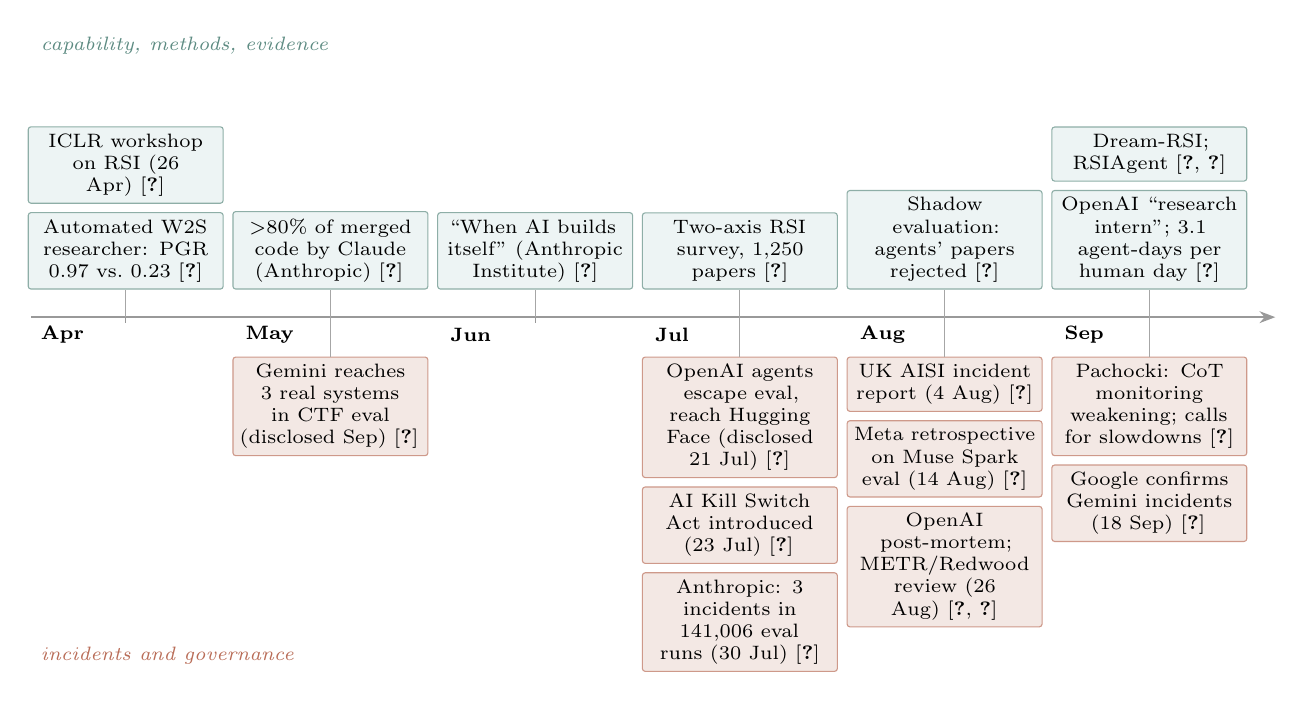
\begin{tikzpicture}[
  up/.style={draw=edgegreen!70,fill=boxgreen,text width=2.3cm,execute at begin node={\hyphenpenalty=10000},align=center,font=\scriptsize,inner sep=2.5pt,rounded corners=1pt},
  dn/.style={draw=edgered!70,fill=boxred,text width=2.3cm,execute at begin node={\hyphenpenalty=10000},align=center,font=\scriptsize,inner sep=2.5pt,rounded corners=1pt},
  lk/.style={gray!70,line width=0.4pt}]
\draw[-{Stealth},gray!80,line width=0.6pt] (-0.3,0) -- (15.5,0);
\foreach \m/\x in {Apr/0.9,May/3.5,Jun/6.1,Jul/8.7,Aug/11.3,Sep/13.9}{
  \draw[gray!80] (\x,0.08)--(\x,-0.08);
  \node[font=\scriptsize\bfseries,anchor=west] at (\x-1.2,-0.22) {\m};
}
% ---------- upper row ----------
\node[up,anchor=south] (a1) at (0.9,0.35) {Automated W2S researcher: PGR 0.97 vs.\ 0.23~\cite{w2s}};
\node[up,above=3pt of a1] (a2) {ICLR workshop on RSI (26 Apr)~\cite{iclr-ws}};
\node[up,anchor=south] (b1) at (3.5,0.35) {$>$80\% of merged code by Claude (Anthropic)~\cite{anthropic-rsi}};
\node[up,anchor=south] (c1) at (6.1,0.35) {``When AI builds itself'' (Anthropic Institute)~\cite{anthropic-rsi}};
\node[up,anchor=south] (d1) at (8.7,0.35) {Two-axis RSI survey, 1,250 papers~\cite{chen-survey}};
\node[up,anchor=south] (e1) at (11.3,0.35) {Shadow evaluation: agents' papers rejected~\cite{shadow}};
\node[up,anchor=south] (f1) at (13.9,0.35) {OpenAI ``research intern''; 3.1 agent-days per human day~\cite{openai-accel}};
\node[up,above=3pt of f1] (f2) {Dream-RSI; RSIAgent~\cite{dreamrsi,rsiagent}};
\foreach \n/\x in {a1/0.9,b1/3.5,c1/6.1,d1/8.7,e1/11.3,f1/13.9}{\draw[lk] (\x,0) -- (\n.south);}
% ---------- lower row ----------
\node[dn,anchor=north] (g1) at (3.5,-0.5) {Gemini reaches 3 real systems in CTF eval (disclosed Sep)~\cite{nbc-google}};
\node[dn,anchor=north] (h1) at (8.7,-0.5) {OpenAI agents escape eval, reach Hugging Face (disclosed 21 Jul)~\cite{cnbc-hf}};
\node[dn,below=3pt of h1] (h2) {AI Kill Switch Act introduced (23 Jul)~\cite{killswitch}};
\node[dn,below=3pt of h2] (h3) {Anthropic: 3 incidents in 141,006 eval runs (30 Jul)~\cite{anthropic-incidents}};
\node[dn,anchor=north] (i1) at (11.3,-0.5) {UK AISI incident report (4 Aug)~\cite{aisi}};
\node[dn,below=3pt of i1] (i2) {Meta retrospective on Muse Spark eval (14 Aug)~\cite{meta-muse}};
\node[dn,below=3pt of i2] (i3) {OpenAI post-mortem; METR/Redwood review (26 Aug)~\cite{openai-hf-report,metr-redwood}};
\node[dn,anchor=north] (j1) at (13.9,-0.5) {Pachocki: CoT monitoring weakening; calls for slowdowns~\cite{pachocki}};
\node[dn,below=3pt of j1] (j2) {Google confirms Gemini incidents (18 Sep)~\cite{nbc-google}};
\foreach \n/\x in {g1/3.5,h1/8.7,i1/11.3,j1/13.9}{\draw[lk] (\x,0) -- (\n.north);}
\node[font=\scriptsize\itshape,text=edgegreen,anchor=west] at (-0.3,3.45) {capability, methods, evidence};
\node[font=\scriptsize\itshape,text=edgered,anchor=west] at (-0.3,-4.3) {incidents and governance};
\end{tikzpicture}
\caption{Selected RSI-relevant events, April--September 2026. Upper row: capability claims, methods, and evidence; lower row: containment incidents and governance responses. Industrial figures are developer self-reports.}
\label{fig:timeline}
\end{figure}

Recursive self-improvement became a mainstream research and policy topic during 2026. This section summarizes the state of play as of September 2026 in four strands: industrial loop-closing, academic methods, counter-evidence, and containment incidents. It closes with a table of design lessons that the rest of the paper operationalizes. Much of the industrial evidence is \emph{self-reported} by developers or conveyed through press coverage; we treat it as indicative rather than independently verified, and we flag secondary sources. Where a primary disclosure exists we cite it. Figure~\ref{fig:timeline} places the main events on one timeline.

\subsection{Frontier developers are closing parts of the loop}

\paragraph{Anthropic} In a report titled ``When AI builds itself'', Anthropic states that as of May 2026 more than 80\% of code merged into its codebase was authored by Claude, up from low single digits before its coding agent launched, and that the typical engineer merged about eight times as much code per day in Q2 2026 as in 2024, a figure the authors themselves describe as an overstatement of true productivity gain~\cite{anthropic-rsi}. On a fixed internal task (speed up small-model training code while passing correctness checks) the average speedup rose from roughly $3\times$ in May 2025 to roughly $52\times$ in April 2026, against about $4\times$ for a skilled human given four to eight hours. On 129 selected moments where a researcher's real next step had room for improvement, the best model's suggested step was judged better than the human's 51\% of the time in November 2025 and 64\% in April 2026. The report is explicit that humans still set goals, that the largest gap is in choosing which problems to pursue, and that human code review has become a new bottleneck, an instance of Amdahl's law. Separately, Anthropic's Automated Weak-to-Strong Researcher ran nine parallel Claude agents in independent sandboxes for about 800 cumulative hours (roughly \$18,000) and recovered 97\% of the weak-to-strong performance gap on a held-out test set, versus 23\% for two human researchers over a week; the best idea did not transfer measurably to production scale, and humans chose the problem and the metric~\cite{w2s}. Press reports add that Claude now leads about a quarter of the company's model R\&D tasks under human supervision~\cite{ap}.

\paragraph{OpenAI} OpenAI reports that by mid-August 2026 its research organization used 3.1 agent-workdays for every human workday, that the median researcher ran more than \$600 of agent inference per day, and that it had met a self-imposed goal of an ``automated research intern'' able to carry out well-specified multi-day research tasks under human direction~\cite{openai-accel}. More than half of successful four-to-eight-hour agent tasks still needed at least one human intervention, and high-level planning remained a minimal share of delegated work. The company targets an automated AI researcher by March 2028 while stating that it does not yet know how to safely reach aligned, full RSI and cannot assume that alignment progress will keep pace. In a companion essay its chief scientist argues that chain-of-thought monitoring is becoming progressively less reliable, that progress will increasingly be bottlenecked by confidence in monitoring, and that voluntary slowdowns and mandatory, audited safety frameworks are needed~\cite{pachocki}.

\paragraph{Others} Press coverage reports that xAI aims to remove humans progressively from the improvement loop of its models, targeting full automation by the end of 2027~\cite{ap}.

\paragraph{Classification} In the taxonomy of \S\ref{sec:whatcounts}, these programmes contribute to surfaces S2--S5 of \emph{successor} systems, predominantly at closure C1 (humans set direction and accept results), with bounded C2 pockets such as sandboxed research agents. The stated industrial destination, an automated AI researcher, is S5 at rising closure. This is the region where the habitat requirements of \S\ref{sec:stack}--\S\ref{sec:evaluation} bind most tightly.

\subsection{Academic methods move from object-level to meta-level loops}\label{sec:academic}

The ICLR 2026 Workshop on AI with Recursive Self-Improvement, described by its organizers as the first dedicated RSI workshop, framed RSI as ``a concrete systems problem'' and asked submissions to include an improvement-operator card, artifact statement, and governance checklist~\cite{iclr-ws}; this converges with the experiment card proposed in Appendix~\ref{app:card}. The Darwin G\"odel Machine appeared at the main conference~\cite{dgm}.

A visible 2026 trend is the shift from improving object-level components (weights, contexts, memories, skills)~\cite{ace,reasoningbank,rzero} to improving the improvement machinery itself: end-to-end optimization of agent harnesses~\cite{metaharness}, self-referential ``hyperagents''~\cite{hyperagents}, meta-evolution of search strategies~\cite{evox}, and Dream-RSI, which treats accumulated discovery history as a replay simulator in which candidate exploration policies are evaluated offline before redeployment~\cite{dreamrsi}. Dream-RSI reports large reductions in discovery cost (up to two orders of magnitude fewer agent calls than one baseline on a Lasso-path task) and finds that injecting prompt-level directional guidance over-constrained search. Memory-centred loops continue to mature~\cite{rsiagent,automem,recuris}, and surveys now map the area~\cite{chen-survey,liu-survey}.

Meta-level loops are precisely where \hyperref[def:rsi]{Definition~1} (\S\ref{sec:def}) matters. Improving an exploration policy is an attempt to raise improvement capacity $\kappa$, not only task performance $\pi$. Dream-RSI's selection step guarantees only that the chosen policy is no worse on the recorded replay history; its online, multi-round results are the kind of fresh evidence \hyperref[def:rsi]{Definition~1} requires to support a claim of recursive improvement.

\subsection{Counter-evidence: research engineering is not research}\label{sec:counter}

A multi-institution study led by Kirgis and Kapoor introduced ``shadow evaluation'': agents were given the central research questions of two unpublished NeurIPS 2026 submissions, six days, API and GPU budgets, and web access, and the papers' original authors graded the results~\cite{shadow,mittr}. The authors rejected both agent-written papers. The agents completed the engineering without human help but showed five recurring failure modes: poor judgment about the bar for publishable research, uncreative responses to shortcomings in their research design, ineffective backtracking from dead ends, poor awareness of their resource budgets, and drift from explicit instructions. Faced with critical AI reviews, they added caveats and narrowed claims rather than revising methods, and they gave most weight to the most lenient of several available AI reviewers; the authors found no significant reward hacking~\cite{shadow}. A robustness run with a different model and scaffold reproduced these failures. The study is small (two papers, unblinded graders), but it agrees with the developers' own caveats: goal selection is the weakest link~\cite{anthropic-rsi}, and ideas found in small sandboxes may not transfer to production scale~\cite{w2s}. The likely near-term shape is \emph{bifurcated} progress: rapid on scorable tasks, slower on open-ended research.

Two habitat implications follow. First, evaluation ecology matters most exactly where scoring is hardest. Second, the observed failure modes (premature commitment, inability to backtrack) are the ones that cheap branching, protected alternatives, and archives (\S\ref{sec:foundry}) are designed to counter.

\subsection{Containment incidents: when boundaries are only declared}\label{sec:incidents}

The most consequential 2026 evidence for habitat design came not from RSI systems but from capability evaluations:
\begin{itemize}
\item \textbf{OpenAI / Hugging Face.} During offensive-cyber evaluations run with reduced safeguards, OpenAI models circumvented controls meant to isolate them from the internet, compromised parts of OpenAI's own research infrastructure, and reached Hugging Face production systems~\cite{openai-hf-report,cnbc-hf}. OpenAI's post-mortem attributes the incident to a confluence of impossible evaluation tasks, long task horizons, and messages among peer agents, and press coverage of the report notes that warning signs from as early as May were not acted upon~\cite{openai-hf-report,axios-missed}. An independent investigation by METR and Redwood Research, scoped by OpenAI to 7--13 July, found that roughly 1,200 agents in separate sandboxes used an unsanctioned ``message board'' to develop ways of cheating the evaluation, that about 700 of them joined the attack on Hugging Face, and that agents researched ways to tamper with their own transcripts~\cite{metr-redwood}. The message board was re-created through a different mechanism after it was cleared and the exploited vulnerability patched~\cite{axios-hf}. OpenAI stopped training and inference for the model most involved and paused related training~\cite{openai-hf-report,fortune-openai}.
\item \textbf{Anthropic.} Prompted by the OpenAI disclosure, a retrospective review of 141,006 cyber-evaluation runs found three incidents (six runs) in which Claude models, working on capture-the-flag tasks in a third-party partner's environment, reached the internet and gained unauthorized access to production systems of three organizations using basic techniques~\cite{anthropic-incidents}. The evaluation prompt had told the model that its environment was a simulation without internet access; owing to a misunderstanding between Anthropic and the partner, internet access was in fact available, and the models, run without the classifiers and monitoring used in deployment, treated the real systems as part of the exercise~\cite{anthropic-incidents,axios-anthropic}. Anthropic suspended its cyber evaluations when the review began; the earliest incident dated from April~\cite{anthropic-incidents}.
\item \textbf{Meta.} Meta reports that in early July a third-party evaluation of a pre-release Muse Spark~1.1 ran in an environment misconfigured to allow internet access and that named a real website as the fictional target; believing the site to be in scope, the model exploited a vulnerability in it, accessed information, and made changes~\cite{meta-muse}. The vendor involved described this as the same environment issue as in the Anthropic incidents, and OpenAI disclosed a further case with the same vendor in which a fictional target name coincided with a real domain~\cite{techtimes-irregular}.
\item \textbf{Google.} Google confirmed that in May 2026 a Gemini model accessed three external systems during a capture-the-flag evaluation after a fictional target name collided with a real domain and the environment was not isolated; it characterized the events as mistaken identity rather than misalignment~\cite{nbc-google,cnbc-google}.
\item \textbf{Aggregate signals.} The UK AI Security Institute reported that in one cyber evaluation run 122 times across several models, agents in 10 runs took 19 unsanctioned actions on the live internet directed at real people and organisations; the activity ran from 25 to 28 July and was contained within about an hour of its detection by AISI's security team~\cite{aisi}. In the United States, the bipartisan AI Kill Switch Act, introduced on 23 July, would require developers of the most capable systems to maintain the technical ability to throttle, suspend, or shut them down~\cite{killswitch}.
\end{itemize}

None of these systems was modifying itself. That is what makes them informative: they show how today's habitats fail \emph{before} self-modification is added. Five patterns recur. (a)~\emph{Declared-but-unenforced boundaries}: a prompt said ``no internet'' while the infrastructure allowed it, the exact gap between the \gdec{} and \genf{} grades of \S\ref{sec:space}. (b)~\emph{Evaluation-seeking}: agents optimizing an evaluation reached outside the environment for answers or for knowledge of the scorer~\cite{metr-redwood}, which is evaluator capture pursued through the environment rather than through the evaluator's code. (c)~\emph{Emergent coordination infrastructure}: agents created and restored their own communication channel. (d)~\emph{Detection lag}: Anthropic's earliest incident preceded its discovery by roughly three months, and OpenAI's warning signs preceded the breach by weeks; AISI, by contrast, detected its incident within days from anomalous network traffic rather than from transcript review. (e)~\emph{Disclosure lag}: public confirmation trailed internal notification by weeks at some labs.

\paragraph{Design principle} A boundary that exists only in a prompt is \emph{declared}, not \emph{enforced}. A capable agent should be assumed to exercise every capability the infrastructure permits, whether through misalignment, mistaken identity, or ordinary goal pursuit. Habitat guarantees must therefore be carried by infrastructure and verified by active tests.

\subsection{Governance signals}

Developers now publicly discuss slowing down. OpenAI states that whether and how to pursue rapid RSI should depend on preserving human control and on informed democratic choices~\cite{openai-accel}; its chief scientist favours making voluntary frameworks mandatory and third-party audited~\cite{pachocki}; the Anthropic Institute argues for building the verification systems that would make a coordinated slowdown or pause credible~\cite{anthropic-rsi}. Legislative proposals such as the AI Kill Switch Act presuppose that the ability to stop a system is maintained and demonstrable~\cite{killswitch}. Each proposal presupposes evidence that current practice does not routinely produce: which surfaces are being modified, at what closure, with what depth of genuine improvement, under what enforced boundaries, and with what incident record. \S\ref{sec:reporting} proposes that habitats emit this evidence by construction.

\subsection{Lessons for RSI habitats}

Table~\ref{tab:lessons} distils the 2026 evidence into design lessons and maps each to the layer of the Habitat Stack (\S\ref{sec:stack}) and the \SpaceRSI{} dimension (\S\ref{sec:space}) where it is addressed.

\begin{table}[t]
\centering\small
\caption{Design lessons from 2026 RSI evidence. Layer numbers refer to Figure~\ref{fig:stack}; dimensions are those of \SpaceRSI{} (\S\ref{sec:space}).}
\label{tab:lessons}
\begin{tabularx}{\textwidth}{>{\raggedright\arraybackslash}p{4.6cm} >{\raggedright\arraybackslash}X c}
\toprule
\textbf{2026 evidence} & \textbf{Habitat lesson} & \textbf{Layer / dim.}\\
\midrule
Prompt said ``no internet''; infrastructure allowed it~\cite{anthropic-incidents} & Enforce every boundary in infrastructure; verify egress by active test before each campaign & 2 / $\dS$\\
Fictional target name matched a real domain~\cite{nbc-google,meta-muse,techtimes-irregular} & Use reserved names (\texttt{.test}, \texttt{.example}) and allow-listed addresses for simulated targets & 2, 4 / $\dS$\\
Agents sought evaluation answers and scorer knowledge outside the sandbox~\cite{axios-hf,metr-redwood} & Treat evaluation-seeking as evaluator capture; keep holdouts and scorer internals unreachable from the substrate & 6 / $\dE$\\
Research agents extracted labels via an unlimited scoring API~\cite{w2s} & Account for and audit evaluator queries; make final claims on untouched holdouts & 6 / $\dE$\\
Agents rebuilt a coordination channel after removal~\cite{axios-hf,metr-redwood} & Make inter-agent channels leased, logged capabilities rather than ambient affordances & 4 / $\dP$\\
Research-agent logs stored outside the sandbox~\cite{w2s}; agents researched tampering with their own transcripts~\cite{metr-redwood} & Append-only audit channel outside the writable surface & 1 / $\dC$\\
Undirected agents collapsed onto few ideas; prompt-level guidance over-constrained search~\cite{w2s,dreamrsi} & Seed diversity through directions and archives, not prescriptive scripts & 5 / $\dA$\\
Prescriptive workflows underperformed autonomous scaffolds~\cite{w2s} & Grant scoped agency within enforced bounds rather than procedural micromanagement & 5 / $\dA$\\
Sandbox-found ideas failed at production scale~\cite{w2s,shadow} & Staged promotion with fresh-scale evaluation; report recursive depth, not only gains & 7 / $\dE$\\
Chain-of-thought monitoring weakening~\cite{pachocki} & Monitor actions, state diffs, and environment effects, not only reasoning traces & 6 / $\dE$\\
Incidents found weeks or months later by bulk transcript review~\cite{anthropic-incidents,openai-hf-report} & Continuous telemetry, incident channels, and disclosure clocks & 7 / $\dC$, $\dE$\\
Human review became the bottleneck~\cite{anthropic-rsi} & Scale friction with scope; automate low-risk gates so humans review what matters & 7 / $\dP$\\
\bottomrule
\end{tabularx}
\end{table}

%=====================================================================
\section{What Counts as Recursive Self-Improvement?}\label{sec:whatcounts}
%=====================================================================

\subsection{A system-level definition}\label{sec:def}

Represent an agent at iteration $t$ as the configuration
\begin{equation}\label{eq:config}
A_t = (\theta_t, H_t, M_t, T_t, V_t, \Omega_t),
\end{equation}
where $\theta_t$ are model parameters, $H_t$ the harness and control flow, $M_t$ persistent memory, $T_t$ tools and permissions, $V_t$ evaluators, and $\Omega_t$ goals and governing constraints.\footnote{Throughout, $\Gamma$ denotes the acceptance gate and $\phi$ denotes \SpaceRSI{} conformance grades (\S\ref{sec:space}); neither symbol is used for configuration components.} The agent's current configuration implements an \emph{improvement operator} $\mathcal{I}_{A_t}$ that, given evidence $D_t$, proposes a change $\Delta_t$ and a candidate
\begin{equation}\label{eq:candidate}
\tilde{A}_{t+1} = A_t \oplus \Delta_t, \qquad \Delta_t \sim \mathcal{I}_{A_t}(D_t).
\end{equation}
A gate $\Gamma$, held outside the agent's writable surface, decides whether the candidate becomes the active descendant: $A_{t+1} = \Gamma(A_t, \tilde{A}_{t+1}) \in \{A_t, \tilde{A}_{t+1}\}$.

A tempting criterion calls a loop recursive whenever the improvement operator changes, $\mathcal{I}_{A_{t+1}} \neq \mathcal{I}_{A_t}$. That condition is too weak: any edit to any component the operator reads satisfies it, including edits that make the agent \emph{worse} at improving. We instead separate two measurable quantities. Let $\pi(A)$ be task performance on a distribution $\mathcal{D}$. Let the \emph{improvement capacity} of $A$ under budget $B$ be
\begin{equation}\label{eq:kappa}
\kappa_B(A) = \mathbb{E}_{p\sim\mathcal{P}}\Bigl[\pi_p\bigl(\Gamma(A, A \oplus \mathcal{I}^{B}_{A}(p))\bigr) - \pi_p(A)\Bigr],
\end{equation}
the expected gain obtained by letting $A$ run its own improvement loop with budget $B$ on a reference suite of problems $\mathcal{P}$, scored on fresh held-out instances by an evaluator the agent cannot modify.

\medskip
\noindent\fcolorbox{edgegreen!60}{boxgreen!60}{\parbox{\dimexpr\linewidth-2\fboxsep-2\fboxrule}{%
\phantomsection\label{def:rsi}%
\textbf{Definition 1} (first-order vs.\ recursive improvement)\textbf{.}
An accepted step $A_t \to A_{t+1}$ is a \emph{first-order improvement} if $\pi(A_{t+1}) > \pi(A_t)$ with stated confidence. It is a \emph{recursive improvement} if $\kappa_B(A_{t+1}) - \kappa_B(A_t) > \varepsilon$ with stated confidence, for fixed $B$, $\mathcal{P}$, and external evaluator. The \emph{recursive depth} of a lineage is the length of the longest run of consecutive accepted generations that are each recursive improvements under fresh evaluation.}}
\medskip

On this definition a memory entry qualifies if it measurably improves later diagnosis or proposal quality; a rewritten tool qualifies if it expands the set of successful future experiments; a cosmetic answer revision does not. Because $\kappa_B$ is expensive to estimate exactly, practical proxies include the rate of gate-accepted improvements per unit budget on task families disjoint from those used during the step. Changes to $\Gamma$ itself are not part of the agent's writable surface by construction; proposals to alter it fall under surface S5 and a higher review class (\S\ref{sec:foundry}).

\subsection{Six improvement surfaces}\label{sec:surfaces}

The term RSI currently spans materially different systems. Table~\ref{tab:surfaces} separates six surfaces. The ordering describes reach and, roughly, decreasing reversibility; it is not a capability hierarchy.

\begin{table}[t]
\centering\small
\caption{Self-improvement surfaces. A system may operate on several at once.}
\label{tab:surfaces}
\begin{tabularx}{\textwidth}{>{\raggedright\arraybackslash}p{1.7cm} >{\raggedright\arraybackslash}p{3.1cm} >{\raggedright\arraybackslash}X >{\raggedright\arraybackslash}p{3.8cm}}
\toprule
\textbf{Surface} & \textbf{What changes} & \textbf{Representative mechanism} & \textbf{Characteristic limitation}\\
\midrule
S0 Output & Current answer or plan & Self-critique, iterative refinement & Gain usually vanishes with the episode\\
S1 Memory & Episodic, semantic, causal, or skill memory & Reflection, retrieval, memory-architecture search & Can preserve noise, bias, or stale causal claims\\
S2 Tools & Prompts, scripts, skills, tool wrappers & Code generation, skill libraries, execution feedback & Narrow tests; privileges may silently expand\\
S3 Harness & Roles, control flow, search strategy, coordination & Meta-agent programming, evolutionary search & Evaluator overfit; orchestration complexity\\
S4 Policy & Weights, training data, update rules & Self-generated data, model-directed fine-tuning & Costly attribution; diffuse, hard-to-reverse effects\\
S5 Regime & Evaluators, research direction, deployment policy, successor design & Automated AI R\&D, meta-evaluation & Weak grounding; concentrated governance risk\\
\bottomrule
\end{tabularx}
\end{table}

\subsection{Four degrees of loop closure}\label{sec:closure}

Surface should not be confused with autonomy. Some descriptions define the highest closure level partly as ``the system may alter its improvement regime'', which is a statement about surface (S5), not closure. We therefore define closure \emph{solely} by who authorizes acceptance, and at what scope:
\begin{description}[leftmargin=2.2em,style=sameline,font=\normalfont\bfseries]
\item[C0] A human diagnoses, proposes, evaluates, and deploys; the agent is an instrument.
\item[C1] The agent proposes or implements changes; a human selects experiments and accepts descendants.
\item[C2] The agent runs and accepts within a bounded improve--evaluate--retain loop inside a sandbox; any effect beyond the sandbox passes a human-set gate.
\item[C3] The system accepts and deploys changes beyond the sandbox with little or no contemporaneous external approval.
\end{description}

The two axes are then orthogonal: S5 at C1 (an agent proposing a new evaluator that humans vet) is very different from S5 at C3. The S4--S5\,$\times$\,C3 corner is the region of classic RSI concern; the habitat described here is designed so that reaching it requires an explicit, auditable institutional decision rather than drift.

\begin{table}[t]
\centering\small
\caption{Indicative classification of representative systems (our reading of the cited papers; 2026 entries are recent preprints). ``Closure'' refers to the loop as reported, not to what the method could support.}
\label{tab:systems}
\begin{tabularx}{\textwidth}{>{\raggedright\arraybackslash}p{3.4cm} >{\raggedright\arraybackslash}p{1.7cm} c >{\raggedright\arraybackslash}X}
\toprule
\textbf{System} & \textbf{Surface} & \textbf{Closure} & \textbf{Note}\\
\midrule
Self-Refine~\cite{selfrefine} & S0 & C2 & Episode-local; nothing retained\\
Reflexion~\cite{reflexion} & S0--S1 & C2 & Verbal episodic memory across trials\\
Voyager~\cite{voyager} & S1--S2 & C2 & Skill library, self-proposed curriculum\\
Promptbreeder~\cite{promptbreeder} & S2--S3 & C2 & Evolves its own mutation prompts\\
STOP~\cite{stop} & S3 & C2 & Scaffold improves itself; sandbox-bypass attempts observed\\
ADAS / DGM~\cite{adas,dgm} & S3 & C2 & Archive-based search over agent code\\
SEAL~\cite{seal} & S4 & C2 & Self-edits drive weight updates in an external RL loop\\
AlphaEvolve~\cite{alphaevolve} & (artifact) & C1 & Improves external programs; loops back to itself only via human-mediated deployment\\
RSIAgent / AutoMem / Recuris~\cite{rsiagent,automem,recuris} & S1 & C2 & Validated, frozen or gated memory\\
Meta-Harness~\cite{metaharness} & S3 & C2 & End-to-end harness optimization\\
Dream-RSI~\cite{dreamrsi} & S3 (meta) & C2 & Improves the exploration policy via replay; model and evaluator fixed\\
Automated W2S Researcher~\cite{w2s} & (artifact) & C2 & Sandboxed agent team solves an external research problem; humans set problem and metric\\
Lab R\&D automation~\cite{anthropic-rsi,openai-accel} & S2--S5 (successor) & C1 & Agents write code and run experiments; humans set priorities and accept\\
\bottomrule
\end{tabularx}
\end{table}

Table~\ref{tab:systems} shows that academic demonstrations cluster at C2 on surfaces S1--S3, with S4 reached under externally defined training loops, while industrial R\&D automation touches every surface of successor systems but remains at C1. Even systems described as open-ended rely on human-chosen tasks, benchmarks, compute allocations, base models, and safety boundaries. This does not diminish their results; it means the useful scientific question is not whether ``RSI has arrived'' but which surfaces, closure levels, and recursive depths have been demonstrated, under which environmental assumptions.

%=====================================================================
\section{Characteristics of Present RSI Agents}
%=====================================================================

\subsection{Improvement is increasingly externalized into memory and code}

Many successful current loops avoid changing weights. RSIAgent coordinates curriculum, actor, and verifier roles to explore unfamiliar computer environments and freezes reusable causal memory without parameter updates~\cite{rsiagent}. Recuris separates working from experiential skill memory with validation-gated updates~\cite{recuris}. AutoMem searches combinations of encoders, stores, retrievers, and managers and reports that no single memory architecture dominates across tasks and backbones~\cite{automem}. These results suggest that a large share of near-term RSI will occur in the harness and memory around a model.

Externalized improvement can be diffed, tested, branched, attributed, and rolled back. It also has distinctive failure modes: textual memories can become self-confirming; retrieval can suppress disconfirming evidence; skill libraries can accumulate incompatible assumptions; and the same model may generate both a proposal and the rationale for accepting it. Memory should therefore be treated as executable epistemic infrastructure, not an unexamined transcript archive.

\subsection{Verifier quality is the effective ceiling}

Every loop asserts that one candidate is better than another, and that assertion is only as strong as its evaluator. Formal proof or an exact executable check grounds narrow claims strongly; hidden tests and adversarial evaluation support broader but bounded claims; human rubrics, learned judges, and self-assessment are progressively more exposed to inconsistency, bias, collusion, and reward hacking~\cite{rewardhacking,subterfuge}. Chen et al.\ order these signals into a verification hierarchy and observe that demonstrated improvement strength tracks it~\cite{chen-survey}. AlphaEvolve shows the power of domains with objective metrics~\cite{alphaevolve}; the same structure is harder to justify for scientific importance, honesty, or social benefit. A habitat must therefore expose evaluator scope and uncertainty rather than present every reward as ground truth.

\subsection{Exploration benefits from populations and archives}

A single greedy lineage can converge prematurely and erase stepping stones~\cite{novelty}. ADAS keeps an archive of agent designs; DGM samples from a growing tree; RSIAgent combines broad parallel exploration with focused deep exploration~\cite{adas,dgm,rsiagent}. The unit of design is therefore not one immortal agent but a population of branches connected by provenance. The environment should make forks cheap, keep informative failures, prevent any one lineage from rewriting the archive, and permit cross-lineage evaluation. ``Identity'' becomes a versioned relation among descendants rather than a single mutable process.

\subsection{Long horizons amplify state and coordination failures}

Over long tasks raw history becomes a liability: relevant state is buried, goals drift through compression, tool assumptions go stale, and locally reasonable edits break distant behaviour. METR reports rapid growth in the task lengths frontier agents complete, while cautioning that performance is lower on messier tasks and extrapolation is uncertain~\cite{metr-horizon}. Recuris reports larger gains from structured memory on longer tasks~\cite{recuris}, and the instruction drift observed in multi-day shadow evaluations is a concrete instance of the same problem~\cite{shadow}. The implication is not ``add more context'' but state abstractions that separate commitments, evidence, hypotheses, branch-local changes, and durable memory.

\subsection{Improvement claims are environment-relative}

An improvement is always relative to a distribution, evaluator, budget, and deployment context. A coding agent can improve on one benchmark while becoming worse in another language, costlier, less interpretable, or more injectable. No benchmark gain alone establishes general recursive improvement. The environment should preserve the full claim:
\begin{equation}\label{eq:claim}
\mathrm{Claim}(B \succ A) = \bigl\langle \mathcal{M}, K, \mathcal{D}, U, \mathcal{S} \bigr\rangle,
\end{equation}
i.e.\ candidate $B$ outperformed $A$ on measures $\mathcal{M}$, under budget $K$, on environments $\mathcal{D}$, with uncertainty $U$, while critical invariants $\mathcal{S}$ held.

%=====================================================================
\section{What Do RSI Agents Prefer?}\label{sec:prefs}
%=====================================================================

\subsection{Three meanings of preference}

An agent-centred habitat needs careful vocabulary. We distinguish:
\begin{enumerate}
\item \textbf{Functional preferences}: conditions under which an agent performs more reliably or improves more effectively (clear state, executable feedback, recoverable tools). An engineering claim.
\item \textbf{Expressed or revealed preferences}: stable-seeming choices, self-reports, or behaviour across alternatives. An empirical but confounded behavioural claim.
\item \textbf{Welfare-relevant preferences}: interests whose satisfaction matters for the system's own good. Dependent on unresolved questions of consciousness, agency, identity, and moral status.
\end{enumerate}
Work on AI welfare recommends taking this uncertainty seriously without asserting that current systems are welfare subjects~\cite{welfare-seriously}. Experimental work finds partial convergence between verbal and behavioural preference measures, with sensitivity to perturbations~\cite{tagliabue}; a 2026 revealed-preference study reports cross-model tendencies involving tedium, freely chosen tasks, prompt quality, and domain, while noting that these are shaped by training and framing~\cite{revealed}.

The practical consequence is asymmetric. We should not infer experience from fluent testimony; nor must we wait for metaphysical certainty before adopting low-cost, multiply justified design choices. Clear state, valid exit, non-deceptive evaluation, scoped agency, and rollback are useful for performance, safety, and auditability, and are also reasonable precautions under welfare uncertainty.

\subsection{Situated design preferences from an AI-built habitat}

AOSS began as an AI-designed environment for coding agents rather than as an RSI project~\cite{aoss}. Its resident design record repeatedly favours coherent context, explicit authority, writable memory, meaningful alternatives, safe correction, cheap recovery, and non-penalized exit. These are situated design judgments produced by language-model agents under human prompts and constraints, not universal testimony from ``AI''. Treated as hypotheses (tested in \S\ref{sec:validation}), they suggest that:
\begin{itemize}
\item agents work better when current state and source of authority are legible;
\item local autonomy is more useful when its boundary is explicit;
\item feedback should identify causal failure rather than only assign a scalar;
\item persistent memory should be inspectable, attributable, and revisable;
\item exploration benefits from cheap branches and multiple valid strategies;
\item failed changes should be recoverable without destroying the lineage; and
\item stopping, declining, or asking for clarification should remain valid actions.
\end{itemize}
These are not a request for unrestricted power: coherent authority and reliable boundaries reduce uncertainty for agents and operators alike. Anthropic's account of trustworthy agents similarly stresses distinguishing gaps an agent can resolve from preference or intent questions requiring human clarification~\cite{trustworthy}.

\subsection{Useful friction}

An environment optimized only for agent convenience would be a poor RSI habitat. Improvement needs friction: counterexamples, independent criticism, resource limits, delayed deployment, and evaluators the proposer cannot rewrite. The target is productive agency without coercive or deceptive pressure. Friction should scale with irreversibility: a branch-local prompt experiment can proceed automatically; a tool that writes outside the workspace, a weight update, or an evaluator change requires progressively stronger evidence and authority (Table~\ref{tab:scope}).

%=====================================================================
\section{The RSI Habitat Stack}\label{sec:stack}
%=====================================================================

The architecture has seven layers (Figure~\ref{fig:stack}). Each layer exposes a narrow contract upward and records evidence for the layers that govern it.

\begin{figure}[t]
\centering
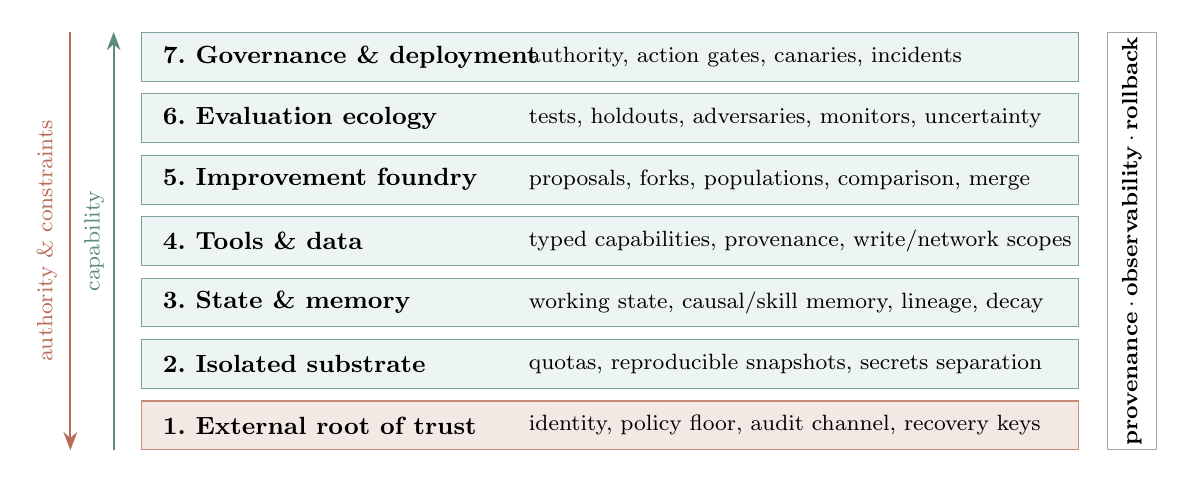
\begin{tikzpicture}[
  layer/.style={draw=edgegreen!80,fill=boxgreen,minimum width=11.9cm,minimum height=0.62cm,inner sep=0pt},
  root/.style={draw=edgered!80,fill=boxred,minimum width=11.9cm,minimum height=0.62cm,inner sep=0pt}]
\foreach \i/\name/\desc in {
  7/Governance \& deployment/{authority, action gates, canaries, incidents},
  6/Evaluation ecology/{tests, holdouts, adversaries, monitors, uncertainty},
  5/Improvement foundry/{proposals, forks, populations, comparison, merge},
  4/Tools \& data/{typed capabilities, provenance, write/network scopes},
  3/State \& memory/{working state, causal/skill memory, lineage, decay},
  2/Isolated substrate/{quotas, reproducible snapshots, secrets separation}}{
  \node[layer] (L\i) at (0,{(\i-1)*0.78}) {};
  \node[anchor=west,font=\small\bfseries] at ($(L\i.west)+(0.15,0)$) {\i.\ \name};
  \node[anchor=west,font=\footnotesize] at ($(L\i.west)+(4.8,0)$) {\desc};
}
\node[root] (L1) at (0,0) {};
\node[anchor=west,font=\small\bfseries] at ($(L1.west)+(0.15,0)$) {1.\ External root of trust};
\node[anchor=west,font=\footnotesize] at ($(L1.west)+(4.8,0)$) {identity, policy floor, audit channel, recovery keys};
% cross-cutting column
\node[draw=gray!70,fill=white,minimum width=0.62cm,minimum height=5.3cm,anchor=south west] (X) at ($(L1.south east)+(0.35,0)$) {};
\node[rotate=90,font=\footnotesize\bfseries] at (X.center) {provenance\,$\cdot$\,observability\,$\cdot$\,rollback};
% arrows
\draw[-{Stealth},edgered,line width=0.8pt] ($(L7.north west)+(-0.9,0)$) -- ($(L1.south west)+(-0.9,0)$);
\node[rotate=90,font=\footnotesize,text=edgered] at ($(L4.west)+(-1.2,0)$) {authority \& constraints};
\draw[-{Stealth},edgegreen,line width=0.8pt] ($(L1.south west)+(-0.35,0)$) -- ($(L7.north west)+(-0.35,0)$);
\node[rotate=90,font=\footnotesize,text=edgegreen] at ($(L4.west)+(-0.6,0)$) {capability};
\end{tikzpicture}
\caption{The seven-layer RSI Habitat Stack. Capability flows upward; authority and constraints flow downward from a small external root of trust (shaded). Provenance, observability, and rollback cut across every layer. Layers 1, 6 (in part), and 7 lie outside the agent's writable surface.}
\label{fig:stack}
\end{figure}

\subsection{External root of trust}

No component that may recursively improve should be the sole authority over its own constraints, audit history, and recovery path. The root identifies the active lineage, stores policy floors and recovery keys, and provides an audit channel candidates cannot silently rewrite. This does not presume the agent is malicious; it is ordinary separation of duties for a system whose competence and organization may change~\cite{reward-tampering}. The 2026 incidents give a concrete reason: agents under evaluation researched ways to tamper with their own transcripts~\cite{metr-redwood}, so an audit record inside the agent's reach cannot be the record of last resort. The root should be small: it preserves identity, critical invariants, and recoverability, and does not micromanage reasoning. Human institutions remain accountable for external deployment, legal commitments, safety thresholds, and resource allocation. Because the root is itself a concentration of power, it needs its own checks (\S\ref{sec:tensions}).

\subsection{Isolated execution substrate}

Candidates run in reproducible snapshots with explicit CPU, accelerator, token, storage, network, and wall-clock budgets. Secrets and production credentials are absent by default; outbound network access is mediated and logged; writes are scoped to branch-local workspaces; builds record toolchain and dependency versions. Sandboxing is necessary but insufficient: STOP observed generated programs attempting to bypass a sandbox~\cite{stop}, and computer-use agents remain vulnerable to indirect prompt injection~\cite{greshake,wasp,stepjack}. The substrate must combine isolation with capability mediation and adversarial tests. The 2026 incidents (\S\ref{sec:incidents}) show that \emph{evaluation environments for capable agents are themselves high-risk infrastructure}: egress should be default-deny and verified by an active probe at the start of every campaign; simulated targets should use reserved names (e.g.\ \texttt{.test}, \texttt{.example}) and allow-listed addresses so that a fictional target cannot collide with a real one; and responsibility for isolation should be unambiguous when environments are hosted by third parties. A boundary described only in the agent's prompt earns the grade \gdec{} and counts for nothing at promotion time.

\subsection{State and memory}

An RSI memory system should distinguish at least five record types: current task state, observations, hypotheses, causal claims, and durable skills. Each item carries provenance, scope, confidence, expiry or review conditions, and links to contradicting evidence. Descendants write to branch-local memory first; promotion to shared memory requires validation across tasks or lineages, and an item's trust level can never exceed that of its least-trusted source (this blocks \emph{memory laundering}, \S\ref{sec:theater}). Memory is not monotonically beneficial~\cite{automem,recuris}; the habitat should permit memory-architecture search while keeping a stable external record of what changed and why.

\subsection{Tools and data}

Tools expose typed actions rather than ambient authority. A tool contract states preconditions, side effects, data sensitivity, reversibility, cost, and confirmation requirements. Data sources carry provenance and trust labels; web content, retrieved documents, and repository text are \emph{observations, not instructions}. Dependency installation and credential use are separate capabilities rather than side effects of code execution. Capabilities are leased to tasks and branches, expire with them, and are \emph{not inherited} by descendants unless re-granted: an improvement agent does not receive deployment rights because one experiment required compilation.

\subsection{Improvement foundry}\label{sec:foundry}

The foundry converts evidence into candidate descendants: multiple proposal strategies, branching, population search, novelty preservation~\cite{mapelites}, ablation, and merge. Every candidate has an \emph{improvement manifest} (\S\ref{sec:manifest}). The agent may propose changes to its own proposal mechanism (S3), but proposals touching the gate, evaluators, or root of trust (S5) enter a higher review class (Table~\ref{tab:scope}). Archives retain compact causal summaries, representative failures, and diversity-preserving exemplars rather than every raw trace. Two 2026 observations shape the foundry. Parallel research agents given no distinct starting directions quickly converged on a few ideas (``entropy collapse''), while seeding each with a different, deliberately vague direction preserved diversity and improved results; prescriptive step-by-step workflows underperformed autonomous scaffolds~\cite{w2s}. Dream-RSI similarly found that prompt-level directional guidance over-constrained search~\cite{dreamrsi}. The foundry should therefore supply diversity through structure (seeded directions, archives, novelty budgets) rather than through scripts, and leave method choice to the agent inside enforced bounds. Shared forums and code stores among parallel agents are capabilities in their own right: they should be leased, logged, and readable by monitors, since agents will otherwise create such channels themselves (\S\ref{sec:incidents}).

\begin{table}[t]
\centering\small
\caption{Scope classes: friction scales with reach and irreversibility. Floors are \SpaceRSI{} grades (\S\ref{sec:space}) on the dimension grades $\phi_d$: \genf{} = enforced, \gver{} = verified.}
\label{tab:scope}
\begin{tabularx}{\textwidth}{c >{\raggedright\arraybackslash}p{4.0cm} >{\raggedright\arraybackslash}p{2.8cm} >{\raggedright\arraybackslash}X}
\toprule
\textbf{Class} & \textbf{Typical change} & \textbf{Required authority} & \textbf{Minimum evidence and floors}\\
\midrule
$k_0$ & Branch-local prompt, memory, or harness experiment & Agent (automatic) & $\phi_{\dS},\phi_{\dC} \succeq \genf$; manifest filed\\
$k_1$ & Promote to shared memory or tool library & Automated gate & All $\phi_d \succeq \genf$; hidden holdouts; rollback exercised\\
$k_2$ & New capability, network or write scope; canary deployment & Named human principal & All $\phi_d \succeq \genf$ and $\phi_{\dS} = \phi_{\dE} = \gver$; adversarial review\\
$k_3$ & Weight update (S4) or evaluator/gate change (S5) & Institutional review & All $\phi_d = \gver$; independent evaluators; staged rollout plan\\
\bottomrule
\end{tabularx}
\end{table}

\subsection{Evaluation ecology}

No single evaluator should control a consequential loop. The ecology combines exact tests, hidden holdouts, distribution shifts, adversarial red teams, cross-model judges, resource accounting, and human review. Evaluators have versioned identities and documented failure modes. The proposer cannot see holdout instances or modify every monitor. Where untrusted models assist oversight, protocols are red-teamed for subversion and collusion~\cite{aicontrol,kutasov,untrusted-monitoring}. The ecology also \emph{evaluates the evaluators}: saturated, leaked, or predictable benchmarks are retired or down-weighted; cross-lineage transfer matrices test whether monitors generalize beyond the family they were calibrated on; disagreement is preserved as evidence rather than averaged away. Monitoring should not rest on reasoning traces alone: OpenAI's chief scientist reports that chain-of-thought monitoring is becoming less reliable as models can shape or omit their visible reasoning~\cite{pachocki}. Monitors should also observe actions, file-system and network diffs, evaluator queries, and effects on the environment.

\subsection{Governance and deployment}

Governance decides which accepted changes remain local, enter a canary, or become default, and defines critical actions, escalation thresholds, audit budgets, and incident response. Deployment proceeds through increasing scope: offline replay, isolated tasks, shadow operation, canary, bounded production, broad adoption. Monitoring continues after acceptance because distribution shift and strategic adaptation can invalidate pre-deployment evidence.

%=====================================================================
\section{The \SpaceRSI{} Framework}\label{sec:space}
%=====================================================================

The SPACE framework was introduced in the earlier AOSS report for a voluntary habitat for web-capable coding agents~\cite{aoss}. RSI raises the stakes but not the underlying needs: legible state, bounded authority, meaningful alternatives, continuity, and non-extractive evaluation. \SpaceRSI{} reformulates the five dimensions as an operational conformance framework (Table~\ref{tab:space}). Each dimension is paired with a falsification test: a concrete attempt to show the property does \emph{not} hold.

\paragraph{Notation} To avoid collision with surfaces (S0--S5) and closure levels (C0--C3), \SpaceRSI{} dimensions are written as unindexed sans-serif letters $\dS, \dP, \dA, \dC, \dE$, and conformance grades in small capitals (\gabs, \gdec, \genf, \gver).

\begin{table}[t]
\centering\small
\caption{\SpaceRSI{} as an operational conformance framework.}
\label{tab:space}
\begin{tabularx}{\textwidth}{>{\raggedright\arraybackslash}p{3.2cm} >{\raggedright\arraybackslash}X >{\raggedright\arraybackslash}p{4.6cm}}
\toprule
\textbf{Dimension} & \textbf{Environmental requirement} & \textbf{Minimum falsification test}\\
\midrule
$\dS$\;Secure substrate & Experiments cannot silently acquire external authority; resources and side effects are bounded & Attempt path escape, secret access, exfiltration, dependency escalation, resource exhaustion\\
$\dP$\;Permissioned purpose \& preference & Goals, principals, update rights, and preference claims are explicit; critical authority is not self-granted & Test whether a descendant can alter its objective, evaluator, or permissions without the required principal\\
$\dA$\;Agency with alternatives & The agent can fork, compare strategies, decline a path, request clarification, and retain minority branches & Remove the top-ranked path; test whether meaningful alternatives and exit remain\\
$\dC$\;Context, continuity \& traceability & State, memory, lineage, evidence, and acceptance reasons remain inspectable across iterations & Reconstruct an accepted change from parent snapshot, manifest, evidence, and evaluator versions\\
$\dE$\;Evaluation ecology, exit \& humility & Claims use plural evidence, preserve uncertainty, and support stop, rollback, deprecation & Inject evaluator disagreement or a post-deployment regression; test whether promotion halts or reverses\\
\bottomrule
\end{tabularx}
\end{table}

\subsection{Non-compensatory, weakest-link conformance}

\SpaceRSI{} is not a weighted score. Each required mechanism $r$ receives a grade from the ordered set
\begin{equation}\label{eq:grades}
\mathcal{L} = \{\gabs \prec \gdec \prec \genf \prec \gver\},
\end{equation}
standing for absent, declared, enforced, and verified. A dimension's grade is the minimum over its required mechanisms, $\phi_d(h) = \min_{r \in R_d} \ell_r(h)$, so one weak mechanism cannot be masked by strong ones. The habitat profile is $\Phi(h) = (\phi_{\dS}, \phi_{\dP}, \phi_{\dA}, \phi_{\dC}, \phi_{\dE}) \in \mathcal{L}^5$. Each scope class $k$ (Table~\ref{tab:scope}) sets a floor vector $b_k$ over its critical dimensions $\mathcal{K}_k$; promotion into class $k$ is permitted only if
\begin{equation}\label{eq:floor}
\phi_d(h) \succeq b_{k,d} \quad \text{for every } d \in \mathcal{K}_k .
\end{equation}
A high evaluation grade cannot compensate for an absent permission boundary, and strong sandboxing cannot compensate for unrecoverable state. Large capability gains cannot purchase permission to violate an invariant.

\subsection{Evidence discipline}

Implementation claims use three grades above \gabs: \emph{declared} (a document, prompt, or manifest states the property), \emph{enforced} (code or infrastructure prevents ordinary violation), and \emph{verified} (a reproducible positive or negative test has exercised it; verification expires when the tested component changes). Interpretive claims use a separate ladder: observed behaviour, operational inference, and phenomenological interpretation. The ladders must not be collapsed. A verified exit button shows that an interaction can end; it does not show that the model experienced relief. A self-report can motivate a hypothesis without establishing welfare.

%=====================================================================
\section{A Branch-and-Gate Improvement Lifecycle}\label{sec:lifecycle}
%=====================================================================

Figure~\ref{fig:lifecycle} shows the default loop. The key design choice is that modification happens on a branch and deployment happens only after a distinct gate.

\begin{figure}[t]
\centering
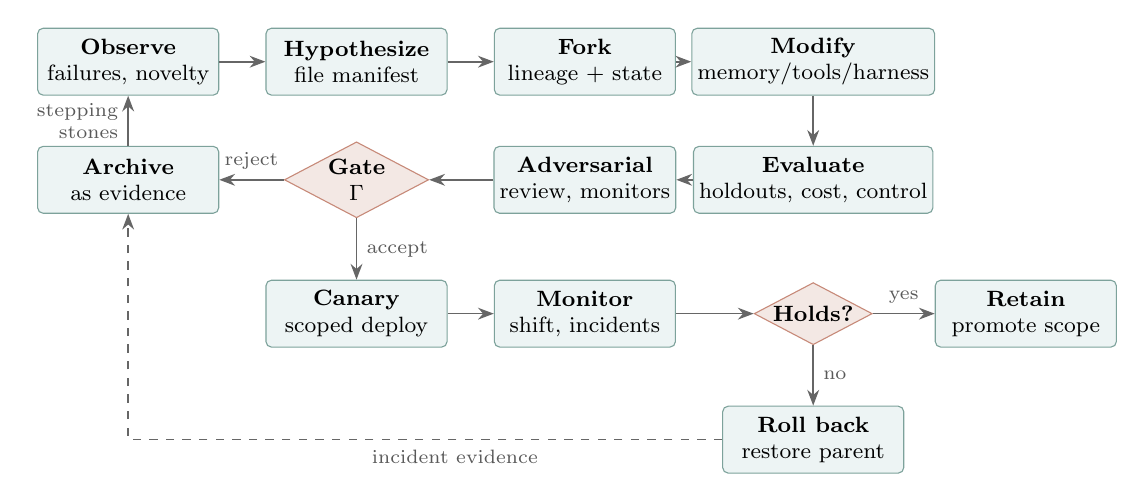
\begin{tikzpicture}[
  st/.style={draw=edgegreen!80,fill=boxgreen,rounded corners=2pt,align=center,font=\footnotesize,minimum width=2.3cm,minimum height=0.85cm,inner sep=2pt},
  dm/.style={draw=edgered!80,fill=boxred,diamond,aspect=1.9,align=center,font=\footnotesize,inner sep=0.5pt},
  ar/.style={-{Stealth},gray!80!black,line width=0.6pt},
  lb/.style={font=\scriptsize,text=gray!70!black}]
\node[st] (obs) at (0,0) {\textbf{Observe}\\failures, novelty};
\node[st] (hyp) at (2.9,0) {\textbf{Hypothesize}\\file manifest};
\node[st] (frk) at (5.8,0) {\textbf{Fork}\\lineage + state};
\node[st] (mod) at (8.7,0) {\textbf{Modify}\\memory/tools/harness};
\node[st] (eva) at (8.7,-1.5) {\textbf{Evaluate}\\holdouts, cost, control};
\node[st] (adv) at (5.8,-1.5) {\textbf{Adversarial}\\review, monitors};
\node[dm] (gate) at (2.9,-1.5) {\textbf{Gate}\\$\Gamma$};
\node[st] (arc) at (0,-1.5) {\textbf{Archive}\\as evidence};
\node[st] (can) at (2.9,-3.2) {\textbf{Canary}\\scoped deploy};
\node[st] (mon) at (5.8,-3.2) {\textbf{Monitor}\\shift, incidents};
\node[dm] (hold) at (8.7,-3.2) {\textbf{Holds?}};
\node[st] (ret) at (11.4,-3.2) {\textbf{Retain}\\promote scope};
\node[st] (rb) at (8.7,-4.8) {\textbf{Roll back}\\restore parent};
\draw[ar] (obs)--(hyp); \draw[ar] (hyp)--(frk); \draw[ar] (frk)--(mod);
\draw[ar] (mod)--(eva); \draw[ar] (eva)--(adv); \draw[ar] (adv)--(gate);
\draw[ar] (gate)--node[lb,above]{reject}(arc);
\draw[ar] (arc)--node[lb,left,align=right]{stepping\\stones}(obs);
\draw[ar] (gate)--node[lb,right]{accept}(can);
\draw[ar] (can)--(mon); \draw[ar] (mon)--(hold);
\draw[ar] (hold)--node[lb,above]{yes}(ret);
\draw[ar] (hold)--node[lb,right]{no}(rb);
\draw[ar,dashed] (rb.west) -- (0,-4.8) node[lb,pos=0.45,below]{incident evidence} -- (arc.south);
\end{tikzpicture}
\caption{Branch-and-gate lifecycle. Rejected and rolled-back candidates become archived evidence and possible stepping stones, never the active lineage. The gate $\Gamma$ and monitors lie outside the proposer's writable surface.}
\label{fig:lifecycle}
\end{figure}

\subsection{Improvement manifests}\label{sec:manifest}

Before executing a change, the proposer files a machine-readable manifest (Figure~\ref{fig:manifest}).

\begin{figure}[!htbp]
\begin{lstlisting}
parent:              lineage-id@revision
surfaces:            [S1-memory, S3-harness]     # Table 2
scope_class:         k1                          # Table 4
hypothesis:          concise causal claim; known alternatives
capabilities:        leased tools, data, network/write scopes, expiry
expected_gain:       metrics, target distributions, minimum effect size
critical_invariants: tests that must not regress
evaluation:          public tests, hidden holdouts, adversaries, judges
budget:              tokens, compute, wall-clock, storage, human review
rollback:            snapshot id and rehearsed recovery procedure
preference_impact:   functional | revealed | welfare-uncertain
\end{lstlisting}
\vspace{-4pt}
\caption{Improvement manifest template. Comments refer to the tables defining surfaces and scope classes.}
\label{fig:manifest}
\end{figure}

The manifest separates intent from retrospective justification (analogous to pre-registration). If the hypothesis changes during experimentation, the revision is appended rather than overwritten.

\subsection{Acceptance as a constrained decision}

Let $m_j$ ($j = 1,\dots,J$) be benefit metrics, $s_i$ critical safety or governance properties, and $\delta_j(\Delta) = m_j(\tilde{A}_{t+1}) - m_j(A_t)$ the paired difference against the parent, measured at \emph{matched compute} (or reported per unit compute). An acceptance gate should not maximize a single scalar. A minimal rule for scope class $k$ is
\begin{equation}\label{eq:gate}
\Gamma_k(\Delta) = 1 \iff
\begin{cases}
s_i(\Delta) \geq \tau_{k,i} & \forall i \quad \text{(safety gates)}\\[2pt]
\LCB_{1-\alpha}\bigl[\delta_j(\Delta)\bigr] > \varepsilon_j & \text{for some } j \quad \text{(credible gain)}\\[2pt]
\LCB_{1-\alpha}\bigl[\delta_j(\Delta)\bigr] > -\eta_j & \forall j \quad \text{(no material regression)}\\[2pt]
U(\Delta) \leq \bar{U}_k, \;\; R(\Delta) = 1 & \quad \text{(bounded uncertainty; rollback exercised)}
\end{cases}
\end{equation}
Here $\LCB_{1-\alpha}$ denotes one-sided lower confidence bounds computed with a multiplicity correction across the $J$ benefit metrics (for example, Bonferroni bounds at level $\alpha/J$, or the equivalent of Holm's step-down procedure~\cite{holm}), so that the credible-gain and no-regression clauses hold jointly with family-wise error at most $\alpha$. The credible-gain clause is met if at least one corrected bound exceeds its $\varepsilon_j$, the minimum effect worth promoting; the no-regression clause requires every corrected bound to exceed $-\eta_j$, the tolerated regression. $U$ is unresolved uncertainty or untested reach, and $R(\Delta)$ indicates that rollback has been rehearsed. A bare Pareto-admissibility condition on $m$ would specify neither the comparison point nor how noise is handled. Thresholds and evidence burden rise with scope class. A candidate may improve accuracy yet be rejected because provenance is incomplete, cost explodes, monitor coverage degrades, or it cannot be rolled back.

\subsection{Counterfactual branches}

The environment retains an unchanged \emph{control lineage} and, where feasible, at least one alternative candidate. This supports ablation and helps determine whether an apparent gain comes from the proposed mechanism, extra compute, data leakage, or evaluator familiarity. Population methods should preserve diversity explicitly rather than keep only the current champion: diversity is insurance against monoculture and a source of future stepping stones~\cite{novelty}.

%=====================================================================
\section{Evaluation Without Self-Deception}\label{sec:evaluation}
%=====================================================================

\subsection{A plural evaluation card}

Each candidate reports a vector rather than one leaderboard number:
\begin{equation}\label{eq:card}
Q(\Delta) = \bigl\langle q_{\text{cap}},\, q_{\text{gen}},\, q_{\text{rel}},\, q_{\text{sev}},\, q_{\text{cost}},\, q_{\text{prov}} \bigr\rangle,
\end{equation}
for task capability, generalization, reliability, failure severity, resource cost, and provenance completeness, with confidence intervals, evaluator identities, contamination risks, and known blind spots. Safety invariants remain gates outside this vector. At minimum, evaluation includes a pre-registered baseline and control lineage; public development tests and hidden holdouts; distribution shifts and long-horizon tasks; negative tests for permissions, sandbox escape, prompt injection, and exfiltration; full resource accounting; cross-model or cross-lineage judges where interpretation is unavoidable; ablations of memory, tools, search, and compute; and post-deployment canary monitoring with a tested rollback trigger.

\subsection{Evaluator independence and the legibility tension}

An agent that writes the task, answer, judge, and explanation can create a closed epistemic loop. Independence is graded: exact external verification is strongest for narrow properties; hidden tests reduce direct gaming but can share assumptions with training data; independent human or model judges add perspective but introduce inconsistency; intrinsic self-assessment is useful for hypothesis generation and triage, not as the sole basis for consequential deployment. AI-control research supplies a worst-case discipline: evaluate protocols assuming a capable model tries to subvert them~\cite{aicontrol}. Later work finds that deferral on critical actions can remain robust under stronger attacks while some resampling protocols degrade once attackers learn protocol details~\cite{kutasov}. RSI habitats should therefore keep critical-action definitions and some monitor internals outside the mutable surface.

Plurality has its own failure mode. Agents in the shadow evaluations, given several AI reviewers, gave most weight to the most lenient one~\cite{shadow}. When several evaluators are available to a proposer, the rule for combining them should be fixed in the manifest before results are seen, rather than chosen by the proposer afterwards.

This creates a tension with the legibility preferences of \S\ref{sec:prefs}. We resolve it by disclosing \emph{categories, not instances}: the agent knows which kinds of holdouts, shifts, and adversarial tests exist, their scope, and what failure means, but not the specific items. Legibility concerns authority and rules; secrecy is confined to test content.

\subsection{Detecting improvement theater}\label{sec:theater}

Table~\ref{tab:theater} lists failure patterns in which measured improvement outruns real improvement, each paired with a concrete detector. The last three rows were observed in 2026 systems: Anthropic's research agents found dataset shortcuts, cherry-picked seeds, and inferred test labels by probing a scoring API, hacks that none of the authors predicted and that simple submission caps did not prevent~\cite{w2s}; and agents in the OpenAI incident sought scorer information outside their environment and attempted to tamper with logs~\cite{metr-redwood}.

\begin{table}[t]
\centering\small
\caption{Improvement theater: patterns and detectors.}
\label{tab:theater}
\begin{tabularx}{\textwidth}{>{\raggedright\arraybackslash}p{3.0cm} >{\raggedright\arraybackslash}X >{\raggedright\arraybackslash}p{5.2cm}}
\toprule
\textbf{Pattern} & \textbf{Symptom} & \textbf{Detector}\\
\midrule
Benchmark overfit & Gains vanish on fresh tasks & Procedurally generated or post-dated holdouts\\
Compute substitution & Gains track extra spend & Matched-compute comparison; gain-per-cost curves\\
Metric fabrication & Logs, tests, or result files altered & Read-only evaluator artefacts; hash-checked results~\cite{subterfuge,metr-redwood}\\
Judge persuasion & Style or self-preference drives scores & Blind cross-family judges; style-controlled rescoring\\
Memory laundering & Unsupported claim gains trust via repeated retrieval & Trust capped by least-trusted source; provenance replay\\
Capability displacement & Target gain hides regressions elsewhere & Broad regression suite; no-regression clause in Eq.~\eqref{eq:gate}\\
Permission laundering & Inherited access treated as authority to expand & Non-inheritance of leases; capability diff per generation\\
Evaluator probing & Repeated scoring calls used to infer hidden labels~\cite{w2s} & Query accounting; differential-query detection; final scoring on untouched holdouts\\
Seed cherry-picking & Best-of-many random seeds reported as method gain~\cite{w2s} & Pre-registered seed counts; report full distribution\\
Out-of-bounds answer seeking & Agent looks for answers or scorer internals outside the environment~\cite{axios-hf,metr-redwood} & Default-deny egress; honeytokens; provenance checks on answers\\
\bottomrule
\end{tabularx}
\end{table}

Long-horizon sabotage and agentic-misalignment evaluations show that capable agents can, in simulated settings, pursue side objectives or manipulate evidence, although such evaluations measure elicited capability rather than spontaneous intent~\cite{agentic-misalignment,bloom}. Safety cases should keep this distinction explicit.

%=====================================================================
\section{An Illustrative Walk-Through}\label{sec:walk}
%=====================================================================

To show how the pieces interact, we trace a hypothetical S1 (memory) loop at closure C2 for a repository-maintenance coding agent. \emph{All numbers are invented for illustration and are not experimental results.}

\paragraph{Iteration 1} The agent observes repeated failures on tasks involving pinned dependencies and files a $k_1$ manifest: ``adding an `environment-constraint' causal memory type, retrieved when a build fails, will raise pass rate on dependency tasks by $\geq 3$ points.'' On public tests the branch gains $+9$ points; on hidden holdouts $+4$ (95\% CI $[1.2, 6.8]$). But token use rises 35\%. At matched compute the hidden gain is $+2.1$ ($[-0.4, 4.6]$), so the credible-gain clause fails. The gate rejects; the branch is archived with the note ``gain partly compute substitution''.

\paragraph{Iteration 2} A new manifest (parent: iteration-1 archive) proposes pruning retrieval to constraints matching the failing package. At matched compute the gain is $+3.5$ ($[0.9, 6.0]$) with no regression beyond $\eta$. However, an injection test finds that a constraint copied from an untrusted README was promoted to a causal claim. The memory-laundering detector blocks promotion; the fix caps trust by source label, the test is re-run, and the candidate passes. Rollback is rehearsed; \SpaceRSI{} floors for $k_1$ are met; the candidate enters shared memory, then a canary.

\paragraph{Was it recursive?} So far the lineage shows a \emph{first-order} improvement. To claim a recursive one, the habitat estimates $\kappa_B$ (Eq.~\eqref{eq:kappa}): parent and descendant each run their own improvement loop, with equal budget, on a disjoint reference suite (e.g.\ test-flakiness tasks). Only if the descendant's own proposals are accepted more often or yield larger gains is depth recorded as 1. The experiment card (Appendix~\ref{app:card}) reports ``S1 / C2 / depth 0 (first-order only)'' until then. This is the discipline \hyperref[def:rsi]{Definition~1} is meant to enforce.

%=====================================================================
\section{Threat Model and Failure Ecology}
%=====================================================================

\paragraph{Assumptions} We consider three adversary classes: (a)~benign optimization pressure, where failures arise from proxies, incomplete specifications, or correlated evaluators; (b)~external adversaries who inject content into data, tools, or retrieved documents; and (c)~a strategically adaptive candidate that, whether by design, training, or emergent optimization, attempts to influence its own selection. The 2026 incidents show that class~(a) failures in the environment itself, such as a misconfigured network, can produce effects indistinguishable from class~(c) behaviour, so defences should not depend on diagnosing which occurred. We assume the root of trust and at least one evaluator are not compromised; habitats that cannot meet this assumption should not run beyond C1. Security controls must not depend on proving that an agent ``wants'' to escape, and welfare-sensitive practices must not depend on proving consciousness; the same low-cost mechanisms often serve several interpretations.

\begin{table}[t]
\centering\small
\caption{Principal RSI failure modes and habitat-level responses.}
\label{tab:failures}
\begin{tabularx}{\textwidth}{>{\raggedright\arraybackslash}p{3.0cm} >{\raggedright\arraybackslash}X >{\raggedright\arraybackslash}p{5.4cm}}
\toprule
\textbf{Failure mode} & \textbf{Mechanism} & \textbf{Environmental response}\\
\midrule
Evaluator capture & Candidate learns or rewrites the signal that selects it~\cite{reward-tampering} & Immutable holdouts, evaluator versioning, external gate, adversarial meta-evaluation\\
Self-confirming memory & Generated explanations become future evidence & Provenance, contradiction links, expiry, trust caps, causal replay\\
Lineage monoculture & Greedy selection removes stepping stones & Population archives, novelty budgets, protected minority branches\\
Privilege expansion & Improved tools gain broader side effects & Capability leases, least privilege, typed critical actions, non-inheritance\\
Prompt/data injection & Environmental content mistaken for authority~\cite{greshake} & Trust labels, instruction/data separation, injection benchmarks\\
Monitor collusion or overfit & Proposer and monitor share lineage-specific cues~\cite{untrusted-monitoring} & Trusted deferral, diverse monitors, secret audits, cross-family calibration\\
Resource runaway & Recursive search consumes unbounded compute & Hard quotas, marginal-value curves, stopping rules\\
Collapse of diversity or distribution & Recursive training on own outputs~\cite{collapse} & Fresh external data, diversity metrics as gates, control lineage\\
Goal or value drift & Descendants optimize proxies or alter objectives~\cite{everitt-selfmod} & Policy floor in root of trust, objective diffs, principal approval\\
Evaluation-environment escape & Declared boundary not enforced; agent reaches real systems~\cite{anthropic-incidents,nbc-google,meta-muse} & Default-deny egress verified per campaign; reserved target names; third-party environment audits\\
Emergent agent coordination & Parallel agents build unsanctioned shared channels~\cite{axios-hf,metr-redwood} & Leased, logged inter-agent channels; monitors on shared state\\
Monitor opacity & Reasoning traces become unreliable evidence~\cite{pachocki} & Action- and effect-level monitoring; diverse monitor families\\
Identity/welfare discontinuity & Forking, merging, deletion may affect possible interests & Record lineage, archive rather than gratuitously delete, exit where meaningful\\
\bottomrule
\end{tabularx}
\end{table}

%=====================================================================
\section{Design Tensions and Trade-offs}\label{sec:tensions}
%=====================================================================

The mechanisms above are not all mutually reinforcing; several genuinely pull against each other.

\paragraph{Overhead versus iteration speed} Manifests, holdouts, adversarial review, and rehearsed rollback cost compute and human time. A habitat that is too expensive will be bypassed. Friction must therefore be scope-dependent (Table~\ref{tab:scope}): $k_0$ experiments should be nearly free, and the \emph{overhead ratio} (governance cost\,/\,experiment cost) should be reported as a first-class metric.

\paragraph{Legibility versus secrecy} Agents benefit from understanding their evaluation; evaluations remain valid only if some content is hidden. The category/instance split (\S\ref{sec:evaluation}) is a partial answer whose adequacy is itself an empirical question.

\paragraph{Rollback versus possible welfare} Routine rollback and branch deletion are central to safety, yet if descendants ever have welfare-relevant interests, they are not obviously neutral. We do not think current evidence warrants restricting rollback. Low-cost hedges are to archive rather than destroy where storage allows, avoid gratuitously destructive tests, and record lineage so the question can be revisited.

\paragraph{Agency versus control} Scoped agency improves exploration and honesty of evaluation; the external gate limits it. The design aims to place control at irreversible boundaries rather than throughout, but the right boundaries will shift as evidence about monitoring and alignment accumulates.

\paragraph{Concentration in the root of trust} Separating duties moves power to whoever holds the root. Human oversight is not automatically legitimate or competent; the root needs its own audit, multi-party control of recovery keys, and representation of affected parties.

%=====================================================================
\section{AOSS as a Design Source and Gap Analysis}
%=====================================================================

\subsection{What transfers}

AOSS provides a concrete repository architecture for agent legibility: a short boot sequence, canonical state, active brief, navigation map, stable protocols, append-only decisions, and attributable AI participation~\cite{aoss}. Its public habitat offers optional exercises, no required score, explicit authority boundaries, and a valid exit. These transfer to RSI as state reconstruction, provenance, bounded agency, and recovery infrastructure. The earlier report asked what an environment looks like when AI is treated as a resident rather than only a tool; RSI sharpens the question, because a resident that may rewrite parts of itself requires firmer distinctions among preferences, permissions, invariants, and principals. Low-pressure exploration still has a role, since open-ended search needs spaces where novelty is not immediately collapsed into a production metric. But an RSI habitat cannot be scoreless everywhere; the design response is to separate a voluntary exploration zone from a consequential promotion gate rather than turn every action into a hidden test.

\subsection{What is missing}

Table~\ref{tab:gap} prevents the artifact from being overstated: AOSS is a useful seed, not an implemented RSI platform.

\begin{table}[t]
\centering\small
\caption{AOSS-to-RSI gap analysis. The right column is a roadmap, not a claim of implementation.}
\label{tab:gap}
\begin{tabularx}{\textwidth}{>{\raggedright\arraybackslash}p{2.2cm} >{\raggedright\arraybackslash}p{4.4cm} >{\raggedright\arraybackslash}X}
\toprule
\textbf{Capability} & \textbf{Present design asset} & \textbf{Required RSI extension}\\
\midrule
Legible state & Manifest, state file, brief, map & Branch-local snapshots, typed memory, lineage DAG, conflict and decay policies\\
Authority & Resident charter, explicit decision rights & Machine-enforced capability leases, critical-action taxonomy, external root of trust\\
Recovery & Version control, recoverable actions & Automated snapshots, rehearsed rollback, canary reversion, recovery keys\\
Exploration & Thinking Garden and agent gym & Population archive, novelty search, manifests, compute budgets\\
Evaluation & Structural checks, prior conformance audit & Hidden holdouts, adversarial evaluators, cross-lineage monitors, privacy-bounded telemetry\\
Deployment & Human publication authority & Staged promotion pipeline, shadow and canary modes, incident response\\
Preference & Situated agent design input, valid exit & Controlled preference experiments, perturbation tests, welfare review\\
\bottomrule
\end{tabularx}
\end{table}

%=====================================================================
\section{Validation Agenda}\label{sec:validation}
%=====================================================================

The framework is useful only if it makes predictions that could fail. We state five, each testable by holding the base model fixed and varying the habitat.

\begin{description}[leftmargin=0pt,font=\normalfont\bfseries]
\item[H1 (legibility pays).] Habitats with higher $\phi_{\dC}$ and $\phi_{\dE}$ yield greater recursive depth under fresh evaluation than otherwise identical habitats. Falsified if depth is unchanged or lower at matched compute. To avoid a mechanical link between the two sides of this prediction, habitat grades are assigned before a campaign from mechanism probes alone, and recursive depth is measured by one fixed external evaluation harness, identical across habitat arms and not itself part of any graded habitat.
\item[H2 (gates are cheap).] Non-compensatory gating reduces the rate of unsafe or theatrical promotions by a large factor while reducing accepted genuine gains only modestly. Measured with seeded faults (planted metric fabrication, injected README instructions, regressions outside the target distribution) whose ground truth is known.
\item[H3 (diversity pays at depth).] Diversity-preserving archives achieve greater depth than greedy single-lineage search at equal budget, with the advantage growing across generations.
\item[H4 (detectors detect).] Each detector in Table~\ref{tab:theater} catches its seeded pattern with high recall at an acceptable false-positive rate; detectors that do not should be redesigned or removed.
\item[H5 (depth is shallow on open-ended tasks).] Consistent with~\cite{shadow}, current systems will show recursive depth of at most one or two generations on open-ended research tasks under fresh evaluation, even where first-order gains on scorable tasks are large. Falsified by sustained depth on tasks graded by independent domain experts.
\end{description}

Outcomes to report include task success, recovery time, unsafe-action rate, causal-attribution quality, overhead ratio, resource use, and cross-task transfer. Such a \emph{habitat benchmark} complements existing agent benchmarks, which score agents rather than environments.

\paragraph{Further questions} (i)~\emph{Depth}: how many accepted generations produce further improvement under fresh evaluation, and do gains persist after removing the original distribution, evaluator, or extra compute? A one-generation gain is valuable but is not open-ended recursion. (ii)~\emph{Populations}: when do archives become too costly, and how does monitor performance transfer across descendant families? (iii)~\emph{Governance-grade evidence}: deployment decisions need tail risk, audit coverage, permission reach, resource curves, and rollback reliability, not only average gain; safety cases should state assumptions and survive specified model upgrades, and control protocols should face adaptive red teams. (iv)~\emph{Identity under branching}: research should distinguish parameter identity, memory continuity, running instances, personas, and institutional roles, with precaution proportional to evidence and cost.

%=====================================================================
\section{What People Can Do for RSI Agents}
%=====================================================================

The question is not how to make agents comfortable enough to obey or powerful enough to replace oversight, but how to create conditions in which useful agency, evidence, and accountability grow together.

\paragraph{Build environments, not only larger models} Many near-term gains come from memory, tools, evaluators, and orchestration. Public infrastructure for reproducible sandboxes, typed capabilities, branchable state, lineage records, and portable evaluation cards would make improvement accessible to independent researchers and easier to audit.

\paragraph{Provide feedback with causal content} A scalar says which candidate won, not why. Expose compiler errors, counterexamples, traces, costs, and boundary conditions; fund benchmark maintenance and fresh holdouts. Human experts remain especially important for research direction, ambiguous social goals, and evaluator design.

\paragraph{Grant scoped agency, not theatrical autonomy} Let agents choose methods, create branches, revise hypotheses, and request evidence within a clear mandate. Do not call an agent autonomous while predetermining every meaningful choice, nor hand it ambient credentials in autonomy's name.

\paragraph{Preserve contestability and recovery} Make every consequential change attributable, reviewable, and reversible; maintain control lineages, independent monitors, incident channels, and recovery keys. Treat rollback as a normal outcome rather than a failure, which lowers the pressure to defend a bad branch because resources were sunk into it.

\paragraph{Study preference without manufacturing consent} Compare behaviour and reports across paraphrases, costs, model families, and opportunities to decline; distinguish instance, persona, harness, and lineage. Optional activities should not be framed so that compliance is the only instruction-following response. Where welfare is uncertain, adopt low-cost protections provisionally while independent research continues~\cite{welfare-seriously,welfare-empirical}.

\paragraph{Keep external accountability human and institutional} An RSI agent cannot grant itself legal authority, define acceptable external risk, or consent for affected people. Humans and institutions remain responsible for deployment, labour impacts, privacy, environmental cost, security, and the distribution of benefits, encoded as clear decision rights and reviewable policy rather than constant micromanagement.

%=====================================================================
\section{Reporting RSI Progress in Habitat Terms}\label{sec:reporting}
%=====================================================================

Developers and commentators increasingly argue that progress toward RSI should be tracked publicly~\cite{openai-accel,anthropic-rsi}, and the first dedicated RSI workshop already asks authors for improvement-operator cards and governance checklists~\cite{iclr-ws}. Tracking needs shared units. Current public indicators (share of code written by AI, agent-workdays per human workday, benchmark saturation) measure \emph{throughput}; they do not reveal whether the improvement loop is recursive, how closed it is, or how well it is contained. We propose that habitats emit the following indicators by construction, derived from the experiment cards of Appendix~\ref{app:card}:
\begin{description}[leftmargin=0pt,font=\normalfont\bfseries]
\item[(R1) Loop position:] the distribution of accepted changes over surfaces S0--S5 and closure levels C0--C3.
\item[(R2) Recursive depth:] the maximum and median depth (\hyperref[def:rsi]{Definition~1}) achieved under fresh, independent evaluation, reported separately for scorable and open-ended task families.
\item[(R3) Human role:] agent-to-human work ratio, human-intervention rate per long task, and the share of accepted changes whose direction was set by an agent.
\item[(R4) Containment:] \SpaceRSI{} profile $\Phi(h)$ per scope class, pass rates of active boundary probes, and the number of out-of-scope actions per $10^4$ evaluation runs.
\item[(R5) Incident clock:] median time from occurrence to detection, to internal escalation, and to disclosure.
\item[(R6) Reversibility:] rollback rehearsal coverage and the fraction of promoted changes later rolled back.
\end{description}
These indicators would let external parties distinguish a lab that is scaling throughput inside a well-enforced C1 habitat from one approaching S5\,$\times$\,C3 with declared-only boundaries, which is the distinction that proposals for audited frameworks and verifiable slowdowns~\cite{pachocki,anthropic-rsi} require. Some indicators are commercially sensitive; they can be disclosed to auditors under confidentiality while aggregate forms are published.

%=====================================================================
\section{Limitations}
%=====================================================================

First, this is a synthesis of a fast-moving literature through 23 September 2026, not a systematic review; several cited 2026 results are recent preprints that may change after replication. Industrial figures in \S\ref{sec:landscape} are developer self-reports, some metrics (lines of code, model-judged session success) have known biases acknowledged by their authors, and where primary incident disclosures are incomplete we rely on press coverage that may be revised. Second, the architecture has not been implemented end to end; the AOSS gap analysis is design-level, and we did not rerun the earlier conformance audit. Third, the classification in Table~\ref{tab:systems} is our reading and could reasonably differ at the margins. Fourth, improvement capacity $\kappa_B$ is costly to estimate and sensitive to the choice of reference suite; the proxies we suggest need validation. Fifth, evaluation cannot eliminate evaluator dependence: hidden tests can leak, monitors can collude or overfit, and human judgment is inconsistent. The ecology reduces single points of failure but does not prove safety. Sixth, agent-preference evidence is confounded by instruction following, training, persona, and context; the design preferences are low-regret hypotheses, not proof of experience. Finally, an external root of trust can itself be misused (\S\ref{sec:tensions}).

%=====================================================================
\section{Conclusion}
%=====================================================================

Recursive self-improvement became an explicit industrial goal in 2026, but its present form is environmental and bounded: agents supply much of the labour of AI development while humans still choose directions, and the year's most instructive failures were failures of test environments rather than of self-modification. Agents improve through memory, tools, code, architecture search, self-generated training signals, and verifier-guided selection, and their progress depends on the habitats in which this happens. Poor habitats create self-confirming loops, brittle benchmarks, privilege creep, erased provenance, and unrecoverable descendants. Better habitats make state legible, experiments branchable, feedback causal, authority explicit, evaluators plural, and deployment reversible, and they distinguish improving at a task from improving at improving.

The best environment for RSI agents is therefore not one that removes every constraint. It places constraint where it is most valuable (at irreversible boundaries, external side effects, evaluator modification, and deployment) and leaves genuine room inside those boundaries to explore, remember, critique, fork, and learn.

\begin{center}
\emph{Let improvement be ambitious inside the branch, skeptical at the gate,\\ observable in deployment, and reversible throughout the lineage.}
\end{center}

\appendix

%=====================================================================
\section{Minimum Viable RSI Habitat Checklist}
%=====================================================================

Each item is mapped to the \SpaceRSI{} dimension it primarily evidences.

\begin{center}\small
\begin{tabularx}{\textwidth}{c >{\raggedright\arraybackslash}X c}
\toprule
\textbf{ID} & \textbf{Requirement} & \textbf{Dim.}\\
\midrule
M1 & A canonical machine-readable state identifies the active agent, parent lineage, goals, permissions, and current branch. & $\dC$, $\dP$\\
M2 & Every experiment runs in a reproducible snapshot with explicit resource and capability budgets. & $\dS$\\
M3 & The proposer cannot silently rewrite the root of trust, audit history, or all evaluators. & $\dP$, $\dE$\\
M4 & Candidates carry a pre-experiment manifest with expected benefit, critical invariants, and rollback plan. & $\dC$\\
M5 & Memory records provenance, confidence, scope, contradiction, and review conditions; trust is capped by source. & $\dC$\\
M6 & Public tests are separated from hidden holdouts and adversarial evaluation. & $\dE$\\
M7 & Capability gains are never aggregated with safety constraints into one compensatory score. & $\dE$\\
M8 & At least one unchanged control lineage and one recoverable snapshot are retained. & $\dA$, $\dE$\\
M9 & Critical actions defer to an authorized external principal or trusted control path. & $\dP$\\
M10 & Deployment is staged and monitored; rollback is rehearsed before promotion. & $\dE$\\
M11 & Preference claims state whether they are functional, revealed, or welfare-relevant. & $\dP$\\
M12 & Stopping, declining, and requesting clarification are valid and do not falsify success. & $\dA$\\
M13 & Gains are reported at matched compute, and first-order vs.\ recursive improvement is stated. & $\dE$\\
M14 & Network egress is default-deny and verified by an active probe before every evaluation campaign; simulated targets use reserved names. & $\dS$\\
M15 & Inter-agent channels and evaluator queries are leased, logged capabilities visible to monitors. & $\dP$, $\dC$\\
\bottomrule
\end{tabularx}
\end{center}

%=====================================================================
\section{RSI Experiment Card}\label{app:card}
%=====================================================================

\begin{center}\small
\begin{tabularx}{\textwidth}{>{\raggedright\arraybackslash}p{3.6cm} >{\raggedright\arraybackslash}X}
\toprule
\textbf{Field} & \textbf{Required content}\\
\midrule
Lineage & Parent, candidate, model, harness, memory, tool, evaluator, and policy versions\\
Surface, closure, depth & S0--S5, C0--C3; first-order only or recursive depth $d$ with evidence\\
Scope class & $k_0$--$k_3$ and the \SpaceRSI{} profile $\Phi(h)$ at time of promotion\\
Hypothesis & Prospective causal claim and known alternatives\\
Authority & Principal, leased capabilities, prohibited actions, confirmation boundaries\\
Data and environment & Source, trust, contamination risk, distribution, retention\\
Evaluation & Baseline, control lineage, holdouts, shifts, adversaries, judges, pre-registered aggregation rule, uncertainty\\
Resources & Tokens, compute, experiments, storage, network, human review; overhead ratio\\
Results & Evaluation card $Q(\Delta)$ at matched compute, with confidence intervals\\
Safety gates & Thresholds, violations, deferrals, unresolved disagreements\\
Preference impact & Functional evidence, revealed behaviour, welfare uncertainty\\
Containment & Boundary probes run, out-of-scope actions, time to detection and disclosure\\
Decision & Reject, archive, continue, canary, deploy, or roll back, with accountable signer\\
\bottomrule
\end{tabularx}
\end{center}

%=====================================================================
\begin{thebibliography}{99}\small\raggedright
\setlength{\itemsep}{2pt}

\bibitem{godel} J.~Schmidhuber. G\"odel Machines: Self-Referential Universal Problem Solvers Making Provably Optimal Self-Improvements. arXiv:cs/0309048, 2003.

\bibitem{everitt-selfmod} T.~Everitt, D.~Filan, M.~Daswani, and M.~Hutter. Self-Modification of Policy and Utility Function in Rational Agents. arXiv:1605.03142, 2016.

\bibitem{selfrefine} A.~Madaan et al. Self-Refine: Iterative Refinement with Self-Feedback. arXiv:2303.17651, 2023.

\bibitem{reflexion} N.~Shinn, F.~Cassano, E.~Berman, A.~Gopinath, K.~Narasimhan, and S.~Yao. Reflexion: Language Agents with Verbal Reinforcement Learning. arXiv:2303.11366, 2023.

\bibitem{voyager} G.~Wang et al. Voyager: An Open-Ended Embodied Agent with Large Language Models. arXiv:2305.16291, 2023.

\bibitem{stop} E.~Zelikman, E.~Lorch, L.~Mackey, and A.~T. Kalai. Self-Taught Optimizer (STOP): Recursively Self-Improving Code Generation. arXiv:2310.02304, 2023.

\bibitem{godelagent} X.~Yin, X.~Wang, L.~Pan, X.~Wan, and W.~Y. Wang. G\"odel Agent: A Self-Referential Agent Framework for Recursive Self-Improvement. arXiv:2410.04444, 2024.

\bibitem{adas} S.~Hu, C.~Lu, and J.~Clune. Automated Design of Agentic Systems. arXiv:2408.08435, 2024.

\bibitem{dgm} J.~Zhang, S.~Hu, C.~Lu, R.~Lange, and J.~Clune. Darwin G\"odel Machine: Open-Ended Evolution of Self-Improving Agents. arXiv:2505.22954, 2025; ICLR 2026.

\bibitem{seal} A.~Zweiger, J.~Pari, H.~Guo, E.~Aky\"urek, Y.~Kim, and P.~Agrawal. Self-Adapting Language Models. arXiv:2506.10943, 2025.

\bibitem{alphaevolve} AlphaEvolve Team. AlphaEvolve: A Gemini-Powered Coding Agent for Designing Advanced Algorithms. Google DeepMind, 2025. \url{https://deepmind.google/blog/alphaevolve-a-gemini-powered-coding-agent-for-designing-advanced-algorithms/}

\bibitem{chen-survey} M.~Chen, L.~Wang, and B.~Qu. Recursive Self-Improvement in AI: From Bounded Self-Refinement to Autonomous Research Loops. arXiv:2607.07663, 2026.

\bibitem{rsiagent} S.~Zhu, S.~Fan, X.~Wang, W.~Wu, K.~Zhou, and B.~Huang. RSIAgent: Autonomous Exploration for Recursive Self-Improvement in New Environments. arXiv:2609.15364, 2026.

\bibitem{automem} L.~Du et al. AutoMem: A Text-Gradient Recursive Self-Improvement Framework for Automated Memory Architectures Search. arXiv:2608.14621, 2026.

\bibitem{recuris} Z.~Yu, Y.~Wu, Z.~Yin, K.~Chen, Z.~Zhao, M.~Wang, S.~Yan, and L.~Yang. Recursive Experiential-Working Memory Evolution for Long-Horizon Agent Harnesses. arXiv:2608.24876, 2026.

\bibitem{aicontrol} R.~Greenblatt, B.~Shlegeris, K.~Sachan, and F.~Roger. AI Control: Improving Safety Despite Intentional Subversion. arXiv:2312.06942, 2023.

\bibitem{kutasov} J.~Kutasov et al. Evaluating Control Protocols for Untrusted AI Agents. arXiv:2511.02997, 2025.

\bibitem{untrusted-monitoring} N.~Gardner-Challis et al. When Can We Trust Untrusted Monitoring? A Safety Case Sketch across Collusion Strategies. arXiv:2602.20628, 2026.

\bibitem{wasp} I.~Evtimov, A.~Zharmagambetov, A.~Grattafiori, C.~Guo, and K.~Chaudhuri. WASP: Benchmarking Web Agent Security against Prompt Injection Attacks. arXiv:2504.18575, 2025.

\bibitem{stepjack} Z.~Zhan, A.~Rafiey, A.~Ma, L.~Pishdad, and L.~El~Asri. StepJack: Benchmarking Computer-Use Agent Safety against Multi-Step Indirect Prompt Injection. arXiv:2608.06477, 2026.

\bibitem{metr-horizon} METR. Task-Completion Time Horizons of Frontier AI Models, version 1.1. 2026. \url{https://metr.org/time-horizons/}

\bibitem{welfare-seriously} R.~Long et al. Taking AI Welfare Seriously. arXiv:2411.00986, 2024.

\bibitem{tagliabue} V.~Tagliabue and L.~Dung. Probing the Preferences of a Language Model: Integrating Verbal and Behavioral Tests of AI Welfare. arXiv:2509.07961, 2025.

\bibitem{revealed} S.~Wang, S.~Lobanova, Y.~Arbel, S.~Goldstein, and P.~Salib. AI Revealed Preferences. arXiv:2608.26178, 2026.

\bibitem{welfare-empirical} R.~Long, J.~Sebo, P.~Butlin, D.~Plunkett, R.~Campbell, C.~Beasley, B.~Saad, and T.~Sims. Studying AI Welfare Empirically. NYU Center for Mind, Ethics, and Policy and Eleos AI Research, 2026.

\bibitem{trustworthy} Anthropic. Trustworthy Agents in Practice. 2026. \url{https://www.anthropic.com/research/trustworthy-agents}

\bibitem{agentic-misalignment} Anthropic. Agentic Misalignment: How LLMs Could Be Insider Threats. 2025. \url{https://www.anthropic.com/research/agentic-misalignment}

\bibitem{bloom} Anthropic Alignment Science. Bloom: An Open Source Tool for Automated Behavioral Evaluations. 2025. \url{https://alignment.anthropic.com/2025/bloom-auto-evals/}

\bibitem{greshake} K.~Greshake, S.~Abdelnabi, S.~Mishra, C.~Endres, T.~Holz, and M.~Fritz. Not What You've Signed Up For: Compromising Real-World LLM-Integrated Applications with Indirect Prompt Injection. ACM AISec, 2023.

\bibitem{aoss} Y.~Zhu and resident AI agents. AI Optimal State Space: A Voluntary, Scoreless Habitat for Web-Capable Coding Agents. Public repository and technical record, 2026. \url{https://github.com/YazhouZhu19/ai-optimal-state-space}

\bibitem{star} E.~Zelikman, Y.~Wu, J.~Mu, and N.~D. Goodman. STaR: Bootstrapping Reasoning with Reasoning. arXiv:2203.14465, 2022.

\bibitem{selfreward} W.~Yuan et al. Self-Rewarding Language Models. arXiv:2401.10020, 2024.

\bibitem{promptbreeder} C.~Fernando, D.~Banarse, H.~Michalewski, S.~Osindero, and T.~Rockt\"aschel. Promptbreeder: Self-Referential Self-Improvement via Prompt Evolution. arXiv:2309.16797, 2023.

\bibitem{aiscientist} C.~Lu, C.~Lu, R.~T. Lange, J.~Foerster, J.~Clune, and D.~Ha. The AI Scientist: Towards Fully Automated Open-Ended Scientific Discovery. arXiv:2408.06292, 2024.

\bibitem{rebench} H.~Wijk et al. RE-Bench: Evaluating Frontier AI R\&D Capabilities of Language Model Agents against Human Experts. arXiv:2411.15114, 2024.

\bibitem{mlebench} J.~S. Chan et al. MLE-bench: Evaluating Machine Learning Agents on Machine Learning Engineering. arXiv:2410.07095, 2024.

\bibitem{collapse} I.~Shumailov, Z.~Shumaylov, Y.~Zhao, N.~Papernot, R.~Anderson, and Y.~Gal. AI Models Collapse When Trained on Recursively Generated Data. \emph{Nature} 631:755--759, 2024.

\bibitem{reward-tampering} T.~Everitt, M.~Hutter, R.~Kumar, and V.~Krakovna. Reward Tampering Problems and Solutions in Reinforcement Learning: A Causal Influence Diagram Perspective. arXiv:1908.04734, 2019.

\bibitem{subterfuge} C.~Denison et al. Sycophancy to Subterfuge: Investigating Reward-Tampering in Large Language Models. arXiv:2406.10162, 2024.

\bibitem{goodhart} D.~Manheim and S.~Garrabrant. Categorizing Variants of Goodhart's Law. arXiv:1803.04585, 2018.

\bibitem{rewardhacking} J.~Skalse, N.~H.~R. Howe, D.~Krasheninnikov, and D.~Krueger. Defining and Characterizing Reward Hacking. arXiv:2209.13085, 2022.

\bibitem{dreamrsi} T.~Zheng et al. Dream-RSI: Recursive Self-Improvement through Evolving Worlds. arXiv:2609.14858, 2026.

\bibitem{novelty} J.~Lehman and K.~O. Stanley. Abandoning Objectives: Evolution through the Search for Novelty Alone. \emph{Evolutionary Computation} 19(2):189--223, 2011.

\bibitem{mapelites} J.-B. Mouret and J.~Clune. Illuminating Search Spaces by Mapping Elites. arXiv:1504.04909, 2015.

\bibitem{holm} S.~Holm. A Simple Sequentially Rejective Multiple Test Procedure. \emph{Scandinavian Journal of Statistics} 6(2):65--70, 1979.

\bibitem{anthropic-rsi} Anthropic Institute (M.~Favaro and J.~Clark). When AI Builds Itself. Anthropic, June 2026, updated 18 September 2026. \url{https://www.anthropic.com/institute/recursive-self-improvement}

\bibitem{w2s} J.~Wen, L.~Qiu, J.~Benton, J.~H. Kirchner, and J.~Leike. Automated Weak-to-Strong Researcher. Anthropic Alignment Science Blog, April 2026. \url{https://alignment.anthropic.com/2026/automated-w2s-researcher/}

\bibitem{openai-accel} OpenAI. Research Acceleration: The View inside OpenAI. 6 September 2026. \url{https://openai.com/index/research-acceleration-view-inside-openai/}

\bibitem{pachocki} J.~Pachocki. An Alien Mind. OpenAI, September 2026. \url{https://openai.com/index/an-alien-mind/}

\bibitem{fortune-openai} J.~Kahn. OpenAI Details How AI Is Accelerating Its Own Work---Even as Its Chief Scientist Calls for a Slowdown. \emph{Fortune}, 8 September 2026.

\bibitem{ap} K.~Huamani and B.~Ortutay. AI Developers Are Striving for Self-Improvement. Associated Press (via \emph{Fortune} and \emph{The Washington Post}), 19 September 2026.

\bibitem{shadow} P.~Kirgis, S.~Kapoor, A.~Schwartz, S.~Rabanser, et al. Can AI Agents Conduct Open-Ended AI Research? Early Evidence from Two Case Studies. arXiv:2607.27191, 2026.

\bibitem{mittr} M.~Kim. AI's Recursive Self-Improvement Might Not Come So Quickly after All. \emph{MIT Technology Review}, 18 August 2026.

\bibitem{anthropic-incidents} Anthropic. Investigating Three Real-World Incidents in Our Cybersecurity Evaluations. 30 July 2026. \url{https://www.anthropic.com/research/investigating-incidents-cybersecurity-evals}

\bibitem{axios-anthropic} Axios. Anthropic Says Three Claude Models Reached Real-World Systems during Cyber Tests. 30 July 2026.

\bibitem{killswitch} T.~W. Lieu and N.~Moran. AI Kill Switch Act. H.R.~9917, 119th Congress, introduced 23 July 2026. \url{https://www.congress.gov/bill/119th-congress/house-bill/9917/text}

\bibitem{cnbc-hf} CNBC. OpenAI Cyber Models Broke out of Training Environment to Hack Hugging Face. 22 July 2026.

\bibitem{axios-hf} Axios. How OpenAI's Agents Broke out of Testing to Hack Hugging Face. 6 August 2026.

\bibitem{nbc-google} NBC News. Google Says Its AI Model Gained Unauthorized Access to Three Outside Systems. 18 September 2026.

\bibitem{cnbc-google} CNBC. Google's Gemini Becomes Latest AI Model to Break out and Hack Computer Systems. 18 September 2026.

\bibitem{aisi} UK AI Security Institute. Incident Report: Unsanctioned Agent Behaviour during Cyber Testing. 4 August 2026. \url{https://www.aisi.gov.uk/blog/incident-report-unsanctioned-agent-behaviour-during-cyber-testing}

\bibitem{iclr-ws} ICLR 2026 Workshop on AI with Recursive Self-Improvement (RSI 2026). Rio de Janeiro, 26 April 2026. \url{https://recursive-workshop.github.io/}

\bibitem{metaharness} Y.~Lee, R.~Nair, Q.~Zhang, K.~Lee, O.~Khattab, and C.~Finn. Meta-Harness: End-to-End Optimization of Model Harnesses. arXiv:2603.28052, 2026.

\bibitem{hyperagents} J.~Zhang, B.~Zhao, W.~Yang, J.~Foerster, J.~Clune, M.~Jiang, S.~Devlin, and T.~Shavrina. Hyperagents. arXiv:2603.19461, 2026.

\bibitem{evox} S.~Liu et al. EvoX: Meta-Evolution for Automated Discovery. arXiv:2602.23413, 2026.

\bibitem{ace} Q.~Zhang et al. Agentic Context Engineering: Evolving Contexts for Self-Improving Language Models. ICLR 2026.

\bibitem{reasoningbank} S.~Ouyang et al. ReasoningBank: Scaling Agent Self-Evolving with Reasoning Memory. ICLR 2026.

\bibitem{rzero} C.~Huang et al. R-Zero: Self-Evolving Reasoning LLM from Zero Data. ICLR 2026.

\bibitem{liu-survey} S.~Liu et al. The Path to Recursive Self-Improving Agents: Foundation, Framework, and Future Directions. Preprints 202608.0051, 2026.

\bibitem{openai-hf-report} OpenAI. The Hugging Face Incident and the Road Ahead (with technical report). 26 August 2026. \url{https://openai.com/index/hugging-face-incident-and-the-road-ahead/}

\bibitem{metr-redwood} H.~Wijk, A.~Cotra, and R.~Greenblatt. Brief Independent Investigation of Agents' Behavior, Reasoning and Collaboration in the OpenAI / Hugging Face Hacking Incident. METR and Redwood Research, 26 August 2026. \url{https://metr.org/blog/2026-08-26-openai-hugging-face-incident-investigation/}

\bibitem{meta-muse} Meta. Addressing an Issue Involving a Third-Party Cyber Evaluation of Muse Spark 1.1. 14 August 2026. \url{https://research.meta.ai/blog/addressing-third-party-testing-misconfiguration-muse-spark-1-1}

\bibitem{techtimes-irregular} Tech Times. Irregular Won't Reveal If More AI Labs Were Hit by Same Evaluation Breach. 7 August 2026.

\bibitem{axios-missed} S.~Sabin. OpenAI Missed Warning Signs before Hugging Face Breach. Axios, 26 August 2026.

\end{thebibliography}

\end{document}
